\documentclass[aspectratio=169,10pt]{beamer}

\usepackage{lmodern}
\usepackage[utf8]{inputenc}
\usepackage[T1]{fontenc}
\usepackage[english]{babel}
\usepackage{amsmath,amssymb,amsfonts}
\usepackage{booktabs}
\usepackage{colortbl}
\usepackage{graphicx}
\usepackage{xcolor}
\usepackage{fontawesome5}
\usepackage{listings}
\usepackage{etoolbox}
\usepackage{tikz}
\usetikzlibrary{positioning, arrows.meta}

\usetikzlibrary{shapes.symbols,shapes.geometric,arrows.meta,positioning,fit,calc,shadows,decorations.pathreplacing,decorations.pathmorphing,shapes.gates.logic.US}

\usetheme{Madrid}
\useinnertheme{rounded}
\useoutertheme{miniframes}

\definecolor{DeepBlue}{RGB}{20,45,85}
\definecolor{AccentOrange}{RGB}{235,90,20}
\definecolor{LightGray}{RGB}{245,246,250}
\definecolor{mygreen}{RGB}{0,153,37}
\definecolor{VSDarkBg}{RGB}{25,25,25}
\definecolor{VSText}{RGB}{245,245,245}
\definecolor{VSBlue}{RGB}{80,180,255}
\definecolor{VSPurple}{RGB}{210,110,210}
\definecolor{VSString}{RGB}{255,140,80}
\definecolor{VSComment}{RGB}{80,220,80}
\definecolor{MacRed}{RGB}{255,95,86}
\definecolor{MacYellow}{RGB}{255,189,46}
\definecolor{MacGreen}{RGB}{39,201,63}
\definecolor{ProgramPurple}{RGB}{124,58,180}
\definecolor{StorageBlue}{RGB}{30,120,200}

\setbeamercolor{palette primary}{bg=DeepBlue,fg=white}
\setbeamercolor{palette secondary}{bg=DeepBlue!80!black,fg=white}
\setbeamercolor{palette tertiary}{bg=DeepBlue!90!black,fg=white}
\setbeamercolor{title}{bg=DeepBlue,fg=white}
\setbeamercolor{frametitle}{bg=DeepBlue,fg=white}
\setbeamercolor{structure}{fg=DeepBlue}
\setbeamercolor{item}{fg=AccentOrange}
\setbeamercolor{alerted text}{fg=AccentOrange}
\setbeamercolor{block title}{bg=DeepBlue,fg=white}
\setbeamercolor{block body}{bg=LightGray,fg=black}
\setbeamercolor{block title example}{bg=AccentOrange,fg=white}
\setbeamercolor{block body example}{bg=AccentOrange!10,fg=black}
\setbeamercolor{vscodelisting}{bg=VSDarkBg}
\setbeamertemplate{blocks}[rounded][shadow=true]
\setbeamertemplate{navigation symbols}{}
\setbeamertemplate{itemize items}[circle]
\setbeamertemplate{enumerate items}[default]
\setbeamercolor{enumerate item}{fg=DeepBlue}
\setbeamerfont{enumerate item}{series=\bfseries}

% ---------- helpers used by the von Neumann section ----------
\tikzset{
  memcell/.style={draw=DeepBlue!60, minimum width=2.6cm, minimum height=0.45cm,
    inner sep=1pt, font=\ttfamily\scriptsize, align=center},
  instrcell/.style={memcell, fill=AccentOrange!18},
  datacell/.style={memcell, fill=StorageBlue!18},
  addr/.style={font=\ttfamily\scriptsize, text=DeepBlue},
}
% numbered orange badge for assumptions
\newcommand{\num}[1]{\tikz[baseline=(n.base)]\node[circle,fill=AccentOrange,text=white,
  inner sep=1.6pt,font=\bfseries\scriptsize] (n) {#1};}
% mini memory stack with the program counter pointing at cell #2
% #1 = x offset, #2 = highlighted cell (0-3), #3 = text of cell 3, #4 = panel heading
\newcommand{\pcstack}[4]{%
  \node[font=\scriptsize\bfseries, text=DeepBlue] at (#1,0.55) {#4};
  \foreach \i/\t in {0/{LOAD 6},1/{ADD 7},2/{STORE 8},3/{#3}} {
    \ifnum\i=#2
      \node[instrcell, minimum width=1.7cm, fill=AccentOrange!45, very thick, draw=AccentOrange] at (#1,{-0.45*\i}) {\t};
    \else
      \node[instrcell, minimum width=1.7cm] at (#1,{-0.45*\i}) {\t};
    \fi
    \node[addr, anchor=west] at ({#1+0.92},{-0.45*\i}) {\i};
  }
  \node[anchor=east, text=AccentOrange, font=\scriptsize\bfseries] at ({#1-0.92},{-0.45*#2}) {PC $\rightarrow$};
}

% ---------- helpers for the dilemma / decision slides ----------
% option card: #1 title, #2 small diagram, #3 advantage, #4 drawback
% (all cards use the same neutral style so the colour does not reveal the answer)
\newcommand{\optcard}[4]{%
  \begin{beamercolorbox}[rounded=true,sep=0.16cm,wd=\linewidth]{block body}
    \centering\small\textbf{#1}\\[0.1cm]
    #2\\[0.1cm]
    \raggedright\footnotesize
    \textcolor{mygreen}{\textbf{+}}\ #3\\[0.06cm]
    \textcolor{MacRed}{\textbf{$-$}}\ #4
  \end{beamercolorbox}}

% progress strip: #1 = number of decisions already made
\newcommand{\progress}[1]{%
  {\centering
  \begin{tikzpicture}
    \foreach \i/\t in {1/Stored program,2/Shared memory,3/Binary,4/Sequential,5/Separate units} {
      \ifnum\i>#1
        \node[draw=DeepBlue!35, dashed, rounded corners=3pt, text=DeepBlue!55, font=\tiny\bfseries,
          minimum width=2.45cm, minimum height=0.36cm, inner sep=1pt] at ({(\i-3)*2.6},0) {\i\ \t};
      \else
        \node[draw=AccentOrange, fill=AccentOrange, rounded corners=3pt, text=white, font=\tiny\bfseries,
          minimum width=2.45cm, minimum height=0.36cm, inner sep=1pt] at ({(\i-3)*2.6},0) {\i\ \t};
      \fi
    }
  \end{tikzpicture}\par}}

% ----- small diagrams used on the dilemma slides -----
\tikzset{smallcell/.style={draw=DeepBlue!60, minimum height=0.27cm, inner sep=0.5pt,
  font=\ttfamily\tiny, align=center}}

\newcommand{\diagWired}{\begin{tikzpicture}
  \node[draw=AccentOrange, very thick, rounded corners=4pt, fill=AccentOrange!12, minimum width=2.5cm,
    minimum height=0.85cm, font=\scriptsize, align=center]
    {\textcolor{AccentOrange}{\faWrench}\ fixed circuit\\[-1pt]program = wiring};
\end{tikzpicture}}

\newcommand{\diagTape}{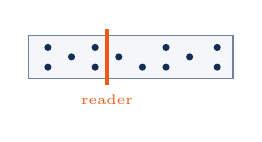
\begin{tikzpicture}
  \draw[draw=DeepBlue!60, fill=LightGray] (0,0) rectangle (2.6,0.55);
  \foreach \x/\y in {0.25/0.15,0.25/0.4,0.55/0.28,0.85/0.15,0.85/0.4,1.15/0.28,1.45/0.15,1.75/0.4,1.75/0.15,2.05/0.28,2.4/0.15,2.4/0.4}
    {\fill[DeepBlue] (\x,\y) circle (0.045);}
  \draw[AccentOrange, very thick] (1.0,-0.08) -- (1.0,0.63);
  \node[font=\tiny, text=AccentOrange, anchor=north] at (1.0,-0.08) {reader};
\end{tikzpicture}}

\newcommand{\diagMemStackSmall}{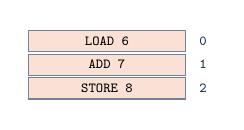
\begin{tikzpicture}
  \node[smallcell, fill=AccentOrange!18, minimum width=2.0cm] at (0,0.3) {LOAD 6};
  \node[smallcell, fill=AccentOrange!18, minimum width=2.0cm] at (0,0) {ADD 7};
  \node[smallcell, fill=AccentOrange!18, minimum width=2.0cm] at (0,-0.3) {STORE 8};
  \node[addr, font=\ttfamily\tiny, anchor=west] at (1.05,0.3) {0};
  \node[addr, font=\ttfamily\tiny, anchor=west] at (1.05,0) {1};
  \node[addr, font=\ttfamily\tiny, anchor=west] at (1.05,-0.3) {2};
\end{tikzpicture}}

\newcommand{\diagTwoMem}{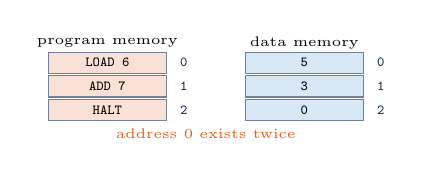
\begin{tikzpicture}
  \node[font=\tiny] at (0,0.55) {program memory};
  \node[font=\tiny] at (2.5,0.55) {data memory};
  \node[smallcell, fill=AccentOrange!18, minimum width=1.5cm] at (0,0.3) {LOAD 6};
  \node[smallcell, fill=AccentOrange!18, minimum width=1.5cm] at (0,0) {ADD 7};
  \node[smallcell, fill=AccentOrange!18, minimum width=1.5cm] at (0,-0.3) {HALT};
  \node[smallcell, fill=StorageBlue!18, minimum width=1.5cm] at (2.5,0.3) {5};
  \node[smallcell, fill=StorageBlue!18, minimum width=1.5cm] at (2.5,0) {3};
  \node[smallcell, fill=StorageBlue!18, minimum width=1.5cm] at (2.5,-0.3) {0};
  \foreach \i in {0,1,2} {
    \node[addr, font=\ttfamily\tiny, anchor=west] at (0.8,{0.3-0.3*\i}) {\i};
    \node[addr, font=\ttfamily\tiny, anchor=west] at (3.3,{0.3-0.3*\i}) {\i};
  }
  \node[font=\tiny, text=AccentOrange] at (1.25,-0.6) {address 0 exists twice};
\end{tikzpicture}}

\newcommand{\diagOneMem}{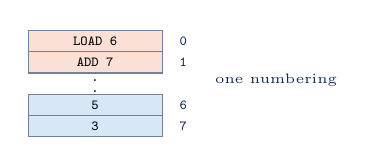
\begin{tikzpicture}
  \node[smallcell, fill=AccentOrange!18, minimum width=1.7cm] (o0) at (0,0.5) {LOAD 6};
  \node[smallcell, fill=AccentOrange!18, minimum width=1.7cm] at (0,0.23) {ADD 7};
  \node[smallcell, draw=none, minimum width=1.7cm] at (0,-0.04) {$\vdots$};
  \node[smallcell, fill=StorageBlue!18, minimum width=1.7cm] at (0,-0.31) {5};
  \node[smallcell, fill=StorageBlue!18, minimum width=1.7cm] at (0,-0.58) {3};
  \node[addr, font=\ttfamily\tiny, anchor=west] at (0.95,0.5) {0};
  \node[addr, font=\ttfamily\tiny, anchor=west] at (0.95,0.23) {1};
  \node[addr, font=\ttfamily\tiny, anchor=west] at (0.95,-0.31) {6};
  \node[addr, font=\ttfamily\tiny, anchor=west] at (0.95,-0.58) {7};
  \node[font=\tiny, text=DeepBlue, anchor=west] at (1.4,0) {one numbering};
\end{tikzpicture}}

\newcommand{\diagDecimal}{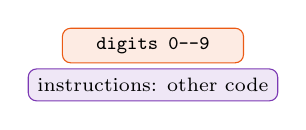
\begin{tikzpicture}
  \node[draw=AccentOrange, fill=AccentOrange!12, rounded corners=3pt, font=\ttfamily\scriptsize, minimum height=0.4cm,
    minimum width=2.3cm] at (0,0.28) {digits 0--9};
  \node[draw=ProgramPurple, fill=ProgramPurple!12, rounded corners=3pt, font=\scriptsize, minimum height=0.4cm,
    minimum width=2.3cm] at (0,-0.22) {instructions: other code};
\end{tikzpicture}}

\newcommand{\diagBinary}{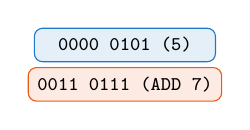
\begin{tikzpicture}
  \node[draw=StorageBlue, fill=StorageBlue!12, rounded corners=3pt, font=\ttfamily\scriptsize, minimum height=0.4cm,
    minimum width=2.3cm] at (0,0.28) {0000 0101 (5)};
  \node[draw=AccentOrange, fill=AccentOrange!12, rounded corners=3pt, font=\ttfamily\scriptsize, minimum height=0.4cm,
    minimum width=2.3cm] at (0,-0.22) {0011 0111 (ADD 7)};
\end{tikzpicture}}

\newcommand{\diagParallel}{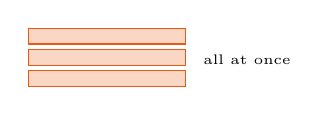
\begin{tikzpicture}
  \foreach \k in {0,1,2} {\draw[fill=AccentOrange!25, draw=AccentOrange] (0,{0.6-0.27*\k}) rectangle (2.0,{0.4-0.27*\k});}
  \node[font=\tiny, anchor=west] at (2.1,0.2) {all at once};
\end{tikzpicture}}

\newcommand{\diagDataflow}{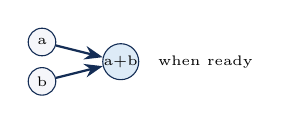
\begin{tikzpicture}[>=Stealth]
  \node[circle, draw=DeepBlue, fill=LightGray, minimum size=0.35cm, inner sep=0pt, font=\tiny] (a) at (0,0.3) {a};
  \node[circle, draw=DeepBlue, fill=LightGray, minimum size=0.35cm, inner sep=0pt, font=\tiny] (b) at (0,-0.2) {b};
  \node[circle, draw=DeepBlue, fill=StorageBlue!15, minimum size=0.4cm, inner sep=0pt, font=\tiny] (c) at (1.0,0.05) {a+b};
  \draw[->, thick, DeepBlue] (a) -- (c); \draw[->, thick, DeepBlue] (b) -- (c);
  \node[font=\tiny, anchor=west] at (1.35,0.05) {when ready};
\end{tikzpicture}}

\newcommand{\diagSequential}{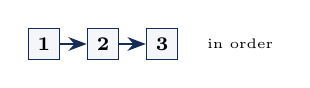
\begin{tikzpicture}[>=Stealth]
  \foreach \k in {1,2,3} {\node[draw=DeepBlue, fill=LightGray, minimum size=0.4cm, inner sep=0pt, font=\scriptsize\bfseries]
    (s\k) at ({0.75*\k-0.75},0.05) {\k};}
  \draw[->, thick, DeepBlue] (s1) -- (s2); \draw[->, thick, DeepBlue] (s2) -- (s3);
  \node[font=\tiny, anchor=west] at (1.95,0.05) {in order};
\end{tikzpicture}}

\newcommand{\diagMonolith}{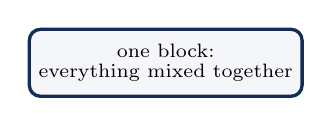
\begin{tikzpicture}
  \node[draw=DeepBlue, very thick, rounded corners=4pt, fill=LightGray, minimum width=2.6cm, minimum height=0.85cm,
    font=\scriptsize, align=center] {one block:\\[-1pt]everything mixed together};
\end{tikzpicture}}

\newcommand{\diagUnits}{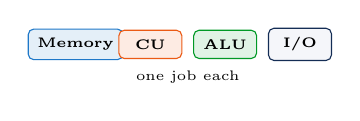
\begin{tikzpicture}
  \node[draw=StorageBlue, fill=StorageBlue!12, rounded corners=2pt, font=\tiny\bfseries, minimum width=0.8cm, minimum height=0.36cm] at (0,0.22) {Memory};
  \node[draw=AccentOrange, fill=AccentOrange!12, rounded corners=2pt, font=\tiny\bfseries, minimum width=0.8cm, minimum height=0.36cm] at (0.95,0.22) {CU};
  \node[draw=mygreen, fill=mygreen!12, rounded corners=2pt, font=\tiny\bfseries, minimum width=0.8cm, minimum height=0.36cm] at (1.9,0.22) {ALU};
  \node[draw=DeepBlue, fill=LightGray, rounded corners=2pt, font=\tiny\bfseries, minimum width=0.8cm, minimum height=0.36cm] at (2.85,0.22) {I/O};
  \node[font=\tiny] at (1.425,-0.2) {one job each};
\end{tikzpicture}}

% ---------- helpers for the CPU section ----------
\tikzset{
  reg/.style={draw=orange!80!black, very thick, fill=yellow!25, rounded corners=2pt,
    minimum width=1.95cm, minimum height=0.55cm, inner sep=2pt, font=\ttfamily\scriptsize, align=center},
  cpuunit/.style={very thick, rounded corners=3pt, minimum width=1.2cm, minimum height=0.6cm,
    inner sep=2pt, font=\scriptsize\bfseries, align=center},
  hot/.style={fill=AccentOrange!45, draw=AccentOrange, very thick},
  hotdata/.style={fill=StorageBlue!40, draw=StorageBlue, very thick},
  hotalu/.style={fill=mygreen!18, line width=1.6pt},
  fetcharrow/.style={-{Stealth}, very thick, DeepBlue, rounded corners=3pt},
  dataarrow/.style={-{Stealth}, very thick, DeepBlue, rounded corners=3pt},
  steplabel/.style={font=\tiny\bfseries, fill=white, inner sep=1pt},
}
% memory with the running example
% #1 highlighted instruction (0-3, -1 = none)  #2 text of cell 8  #3 highlighted data cell (6-8, 0 = none)
\newcommand{\mempanel}[3]{%
  \node[font=\scriptsize\bfseries, text=StorageBlue] at (0,1.8) {Memory};
  \foreach \i/\t in {0/{0001 0110\ \ LOAD 6},1/{0011 0111\ \ ADD 7},2/{0010 1000\ \ STORE 8},3/{0111 0000\ \ HALT}} {
    \ifnum\i=#1
      \node[instrcell, minimum width=2.9cm, hot] (m\i) at (0,{1.35-0.45*\i}) {\t};
    \else
      \node[instrcell, minimum width=2.9cm] (m\i) at (0,{1.35-0.45*\i}) {\t};
    \fi
    \node[addr, anchor=east] at (-1.5,{1.35-0.45*\i}) {\i};
  }
  \node[memcell, draw=none, minimum width=2.9cm] at (0,-0.45) {$\vdots$};
  \foreach \i/\t/\y in {6/{0000 0101\ \ (5)}/-0.9,7/{0000 0011\ \ (3)}/-1.35,8/{#2}/-1.8} {
    \ifnum\i=#3
      \node[datacell, minimum width=2.9cm, hotdata] (m\i) at (0,\y) {\t};
    \else
      \node[datacell, minimum width=2.9cm] (m\i) at (0,\y) {\t};
    \fi
    \node[addr, anchor=east] at (-1.5,\y) {\i};
  }
}
% the CPU, built up step by step
% #1 level: 0 empty, 1 +PC, 2 +IR, 3 +AC, 4 +ALU, 5 +CU   #2 PC   #3 IR   #4 AC   #5 extra ALU style
\newcommand{\cpupanel}[5]{%
  \node[draw=DeepBlue, very thick, rounded corners=6pt, fill=DeepBlue!6, minimum width=4.65cm,
    minimum height=3.85cm, anchor=west] (cpu) at (2.45,-0.2) {};
  \node[font=\scriptsize\bfseries, text=DeepBlue, anchor=north west] at ([shift={(0.1,-0.06)}]cpu.north west) {CPU};
  \ifnum#1>0 \node[reg] (pc) at (3.65,0.95) {\textbf{PC}\ \ #2}; \fi
  \ifnum#1>1 \node[reg] (ir) at (3.65,0.0) {\textbf{IR}\\[-1pt]#3}; \fi
  \ifnum#1>2 \node[reg] (ac) at (3.65,-1.05) {\textbf{AC}\ \ #4}; \fi
  \ifnum#1>3 \node[cpuunit, draw=mygreen, fill=mygreen!18, #5] (alu) at (6.3,-1.05)
    {\textcolor{mygreen!60!black}{\faCalculator}\\[-1pt]ALU}; \fi
  \ifnum#1>4 \node[cpuunit, draw=AccentOrange, fill=AccentOrange!18] (cu) at (6.3,0.5)
    {\textcolor{AccentOrange}{\faCogs}\\[-1pt]CU}; \fi
}
% explanation slide: #1 title, #2 tikz body (memory + CPU), #3 right-hand column
\newcommand{\explainframe}[3]{%
\begin{frame}{#1}
  \begin{columns}[c,onlytextwidth]
    \column{0.58\textwidth}
      \centering
      \begin{tikzpicture}[>=Stealth, scale=0.92, every node/.append style={transform shape}]
        #2
      \end{tikzpicture}
    \column{0.4\textwidth}
      #3
  \end{columns}
\end{frame}}
% boxes for the right-hand column
\newcommand{\defbox}[1]{%
  \begin{beamercolorbox}[rounded=true,sep=0.1cm,wd=\linewidth]{block body example}
    \footnotesize #1
  \end{beamercolorbox}\vspace{0.06cm}}
\newcommand{\stepbox}[2]{%
  \begin{beamercolorbox}[rounded=true,sep=0.09cm,wd=\linewidth]{block body}
    \footnotesize\textbf{#1}\\ #2
  \end{beamercolorbox}\vspace{0.06cm}}
\newcommand{\phasename}[1]{%
  {\centering\footnotesize Name of this phase:\ \colorbox{DeepBlue}{\textcolor{white}{\textbf{#1}}}\par}}
% small tag above the CPU box: which instruction is being executed
\newcommand{\executing}[1]{%
  \node[font=\scriptsize\bfseries, text=AccentOrange, anchor=south east] at ([yshift=1pt]cpu.north east)
    {Executing: \texttt{#1}};}
\newcommand{\statebox}[1]{%
  {\centering\scriptsize\textcolor{DeepBlue}{\textbf{State:}}\ #1\par}}

\lstset{
  language=Python,
  basicstyle=\color{VSText}\ttfamily\footnotesize,
  keywordstyle=\color{VSPurple}\bfseries,
  stringstyle=\color{VSString},
  commentstyle=\color{VSComment}\itshape,
  numbers=left,
  numberstyle=\tiny\color{gray},
  stepnumber=1,
  breaklines=true,
  showstringspaces=false,
  xleftmargin=15pt,
  xrightmargin=5pt,
  frame=none
}

% MARIE assembly: line numbers start at 0, so a line number equals the memory address
\lstdefinelanguage{MARIE}{
  morekeywords={Load,Store,Add,Subt,Input,Output,Halt,Jump,Skipcond,DEC,HEX,ADR,LoadI,StoreI,AddI,JumpI,JnS,Clear,LoadImmi},
  sensitive=false,
  comment=[l]{/},
}
\lstdefinestyle{marie}{language=MARIE, firstnumber=0, basicstyle=\color{VSText}\ttfamily\scriptsize,
  keywordstyle=\color{VSBlue}\bfseries, commentstyle=\color{VSComment}\itshape,
  columns=fixed, basewidth=0.52em, keepspaces=true, breaklines=false, xleftmargin=12pt}

\BeforeBeginEnvironment{lstlisting}{%
  \begin{beamercolorbox}[rounded=true,sep=2mm,wd=\linewidth]{vscodelisting}%
  
\begin{tikzpicture}
    \fill[MacRed] (0,0) circle (3pt);
    \fill[MacYellow] (0.35,0) circle (3pt);
    \fill[MacGreen] (0.70,0) circle (3pt);
  \end{tikzpicture}%
  \vspace{-0.2cm}%
}
\AfterEndEnvironment{lstlisting}{\end{beamercolorbox}}

% =====================================================================
%  Day 2 helpers
% =====================================================================

% ---------- MARIE datapath, drawn like the Data Path view of MARIE.js ----------
% \busdiagram[values]{source}{destination}{extra TikZ}
%   source (Read, blue) and destination (Write, red): ir, out, in, ac, mbr, pc, mar, mem, none
%   values: ir=, out=, in=, ac=, mbr=, pc=, mar=, mem= (contents of M[MAR]), step= (0-7, -1 = none)
\definecolor{ReadBlue}{RGB}{30,150,230}
\definecolor{WriteRed}{RGB}{220,50,80}
\definecolor{BusGreen}{RGB}{60,170,110}
\tikzset{
  dpreg/.style={draw=DeepBlue!80, thick, fill=white, minimum width=1.1cm, minimum height=0.46cm,
    inner sep=1pt, font=\ttfamily\scriptsize},
  dpname/.style={font=\tiny, text=DeepBlue!80, above=0pt, inner sep=1pt},
  dpwire/.style={thin, DeepBlue!18},
  dpmem/.style={draw=StorageBlue, very thick, fill=StorageBlue!12, rounded corners=3pt,
    minimum width=1.3cm, minimum height=0.95cm, font=\scriptsize\bfseries, align=center},
  srcreg/.style={draw=ReadBlue, line width=1.6pt},
  dstreg/.style={draw=WriteRed, line width=1.6pt},
}
\pgfkeys{/dp/.is family, /dp,
  ir/.initial={0000}, out/.initial={0000}, in/.initial={0000}, ac/.initial={0000},
  mbr/.initial={0000}, pc/.initial={000}, mar/.initial={000}, mem/.initial={0000},
  step/.initial={-1}}
\newcommand{\dpv}[1]{\pgfkeysvalueof{/dp/#1}}
\newcommand{\busdiagram}[4][]{%
  \begingroup
  \pgfkeys{/dp, ir=0000, out=0000, in=0000, ac=0000, mbr=0000, pc=000, mar=000, mem=0000, step=-1, #1}%
  \begin{tikzpicture}[>=Stealth]
    \tikzset{bd-mem/.style={}, bd-mar/.style={}, bd-pc/.style={}, bd-mbr/.style={},
      bd-ac/.style={}, bd-ir/.style={}, bd-in/.style={}, bd-out/.style={}, bd-none/.style={}}
    \tikzset{bd-#2/.style={srcreg}}
    \tikzset{bd-#3/.style={dstreg}}
    % ----- control unit -----
    \node[draw=DeepBlue!80, thick, fill=white, minimum width=1.3cm, minimum height=2.95cm,
      anchor=north west] (cu) at (-2.4,2.0) {};
    \node[font=\tiny, text=DeepBlue, anchor=north west, below=1pt] at (cu.south west) {Control unit};
    \node[font=\tiny, text=DeepBlue!80, anchor=east] at (-1.15,1.75) {Read};
    \node[font=\tiny, text=DeepBlue!80, anchor=east] at (-1.15,-0.6) {Write};
    \node[font=\tiny, text=DeepBlue!80, anchor=east] at (-1.15,0.05) {AC<0};
    \node[font=\tiny, text=DeepBlue!80, anchor=east] at (-1.15,-0.15) {AC=0};
    \node[font=\tiny, text=DeepBlue!80] at (-2.0,1.3) {Step};
    \foreach \k in {0,...,7} {
      \pgfmathtruncatemacro{\cur}{\dpv{step}}
      \ifnum\k=\cur
        \fill[ReadBlue] (-2.0,{1.1-0.15*\k}) circle (0.065);
      \else
        \fill[DeepBlue!30] (-2.0,{1.1-0.15*\k}) circle (0.035);
      \fi
    }
    % ----- memory -----
    \node[draw=DeepBlue!80, thick, fill=white, minimum width=1.5cm, minimum height=2.95cm,
      anchor=north west, bd-mem] (mem) at (10.4,2.0) {};
    \node[font=\tiny, text=DeepBlue, anchor=north west, below=1pt] at (mem.south west) {Main memory};
    \node[font=\ttfamily\tiny, text=DeepBlue!80] at (11.15,0.75) {M[MAR]};
    \node[font=\ttfamily\scriptsize] at (11.15,0.5) {\dpv{mem}};
    % ----- faint control wires (one Read and one Write wire per device) -----
    \draw[dpwire] (-1.1,1.75) -- (10.4,1.75);
    \draw[dpwire] (-1.1,-0.6) -- (10.4,-0.6);
    \foreach \x in {0.6,2.0,3.4,4.8,6.2,7.6,9.0} {
      \draw[dpwire] (\x-0.25,1.75) -- (\x-0.25,1.18);
      \draw[dpwire] (\x+0.3,-0.6) -- (\x+0.3,0.72);
    }
    % ----- bus (drawn first, registers on top) -----
    \foreach \x in {0.6,2.0,3.4,4.8,6.2,7.6,9.0}
      \draw[line width=2.6pt, BusGreen] (\x,0.72) -- (\x,-0.35);
    \draw[line width=2.6pt, BusGreen] (0.6-0.045,-0.35) -- (10.4,-0.35);
    % ----- ALU between AC and MBR, with its links and the flag wires to the CU -----
    \draw[thin, DeepBlue!40] (4.45,0.05) -- (-1.1,0.05);
    \draw[thin, DeepBlue!40] (4.45,-0.15) -- (-1.1,-0.15);
    \draw[thick, DeepBlue!70, fill=white] (5.0,0.47) -- (5.42,0.47) -- (5.5,0.37) -- (5.58,0.47) -- (6.0,0.47)
      -- (5.72,0.05) -- (5.28,0.05) -- cycle;
    \node[font=\tiny, text=DeepBlue!80] at (5.5,0.22) {ALU};
    \draw[thick, DeepBlue!60] (5.2,0.72) -- (5.2,0.47);
    \draw[thick, DeepBlue!60] (5.8,0.72) -- (5.8,0.47);
    \draw[thick, DeepBlue!60] (5.5,0.05) -- (5.5,-0.1) -- (4.45,-0.1) |- (4.45,0.72);
    % ----- registers -----
    \foreach \n/\x/\lab in {ir/0.6/IR, out/2.0/OUT, in/3.4/IN, ac/4.8/AC, mbr/6.2/MBR, pc/7.6/PC, mar/9.0/MAR} {
      \node[dpreg, bd-\n] (\n) at (\x,0.95) {\dpv{\n}};
      \node[dpname] at (\n.north) {\lab};
      \coordinate (\n-port) at (\n.south);
      \coordinate (\n-bus) at (\x,-0.35);
    }
    \coordinate (mem-port) at (10.4,-0.35);
    \coordinate (mem-bus) at (10.4,-0.35);
    % IR is decoded by the CU; MAR selects the memory cell
    \draw[thick, BusGreen, -{Stealth}] (ir.west) -- (-1.1,0.95);
    \draw[thick, BusGreen, -{Stealth}] (mar.east) -- (10.4,0.95);
    % ----- active Read and Write signals -----
    \ifstrequal{#2}{none}{}{%
      \ifstrequal{#2}{mem}
        {\draw[line width=1.3pt, ReadBlue, -{Stealth}] (-1.1,1.75) -- (10.4,1.75);}
        {\draw[line width=1.3pt, ReadBlue, -{Stealth}] (-1.1,1.75) -| ($(#2.north)+(-0.25,0)$);}}
    \ifstrequal{#3}{none}{}{%
      \ifstrequal{#3}{mem}
        {\draw[line width=1.3pt, WriteRed, -{Stealth}] (-1.1,-0.6) -- (10.4,-0.6);}
        {\draw[line width=1.3pt, WriteRed, -{Stealth}] (-1.1,-0.6) -| ($(#3.south)+(0.3,0)$);}}
    % ----- the value travelling along the bus -----
    \ifstrequal{#2}{none}{}{\ifstrequal{#3}{none}{}{%
      \draw[line width=3pt, BusGreen] (#2-port) -- (#2-bus) -- (#3-bus) -- (#3-port);
      \draw[line width=1.5pt, white, dash pattern=on 1.5pt off 1.5pt] (#2-port) -- (#2-bus) -- (#3-bus) -- (#3-port);}}
    #4
  \end{tikzpicture}%
  \endgroup}

% legend for the colours of the data path
\newcommand{\dplegend}{%
  {\tiny\textcolor{ReadBlue}{\rule{0.25cm}{0.2cm}}\ \textbf{Read}: puts its value on the bus
  \qquad\textcolor{WriteRed}{\rule{0.25cm}{0.2cm}}\ \textbf{Write}: stores the value from the bus
  \qquad\tikz[baseline=-0.6ex]{\draw[line width=3pt, BusGreen] (0,0) -- (0.5,0);\draw[line width=1.5pt, white, dash pattern=on 1.5pt off 1.5pt] (0,0) -- (0.5,0);}\ the value travelling on the bus}}

% one step of an instruction: data path on top, explanation below
% #1 title, #2 source, #3 destination, #4 values (keys), #5 explanation
\newcommand{\stepframe}[5]{%
\begin{frame}{#1}
  \begin{center}
    \resizebox{0.8\textwidth}{!}{\busdiagram[#4]{#2}{#3}{}}\\[0.02cm]
    \dplegend
  \end{center}
  \vspace{-0.1cm}
  \begin{center}
    \begin{minipage}{0.8\textwidth}
      #5
    \end{minipage}
  \end{center}
\end{frame}}

% ---------- timeline of clock steps ----------
% #1 fetch steps, #2 execute steps, #3 label on the right
\newcommand{\steptimeline}[3]{%
  \begin{tikzpicture}
    \foreach \i in {1,...,#1}
      \node[draw=white, fill=StorageBlue!75, text=white, font=\tiny\bfseries, minimum width=0.62cm,
        minimum height=0.45cm, inner sep=0pt] at ({0.62*(\i-1)},0) {T\the\numexpr\i-1\relax};
    \foreach \i in {1,...,#2}
      \node[draw=white, fill=AccentOrange, text=white, font=\tiny\bfseries, minimum width=0.62cm,
        minimum height=0.45cm, inner sep=0pt] at ({0.62*(#1+\i-1)},0) {T\the\numexpr#1+\i-1\relax};
    \node[anchor=west, font=\scriptsize] at ({0.62*(#1+#2)-0.25},0) {#3};
  \end{tikzpicture}}

% legend for the timeline colours
\newcommand{\timelinelegend}{%
  {\tiny\textcolor{StorageBlue!75}{\rule{0.25cm}{0.2cm}}\ fetch
  \qquad\textcolor{AccentOrange}{\rule{0.25cm}{0.2cm}}\ execute}}

% ---------- small pieces for the addressing-mode slides ----------
\tikzset{
  mcell/.style={draw=DeepBlue!60, minimum width=1.5cm, minimum height=0.42cm, inner sep=1pt,
    font=\ttfamily\scriptsize, align=center, fill=StorageBlue!15},
  mcellhot/.style={mcell, fill=StorageBlue!45, draw=StorageBlue, very thick},
  mcellptr/.style={mcell, fill=ProgramPurple!18, draw=ProgramPurple, very thick},
  instrbox/.style={draw=AccentOrange, very thick, fill=AccentOrange!15, rounded corners=2pt,
    minimum height=0.5cm, inner sep=3pt, font=\ttfamily\scriptsize},
  ptrarrow/.style={-{Stealth}, very thick, DeepBlue},
  valarrow/.style={-{Stealth}, very thick, DeepBlue},
}

% task header box (same look as on Day 1)
% #1 form and time, #2 short instruction
\newcommand{\taskhead}[2]{%
  \begin{beamercolorbox}[rounded=true,sep=0.12cm,wd=\linewidth]{block body example}
    \small\textbf{#1}\\[0.04cm]
    \footnotesize #2
  \end{beamercolorbox}\vspace{0.1cm}}

% highlighted key message at the bottom of a slide
\newcommand{\keymsg}[1]{%
  \begin{beamercolorbox}[rounded=true,sep=0.1cm,wd=\textwidth]{block body example}
    \centering\footnotesize #1
  \end{beamercolorbox}}

% register transfer written in text: \mo{MAR}{PC} gives MAR <- PC
\newcommand{\mo}[2]{\texttt{#1\,$\leftarrow$\,#2}}

% plain listings (x86, RISC-V) without Python highlighting
\lstdefinelanguage{plain}{}
\lstdefinestyle{asm}{language=plain, basicstyle=\color{VSText}\ttfamily\scriptsize, numbers=none,
  columns=fixed, basewidth=0.52em, keepspaces=true, xleftmargin=6pt}

% =====================================================================
%  Day 3 helpers
% =====================================================================

\usetikzlibrary{patterns}
\usepackage{multirow}
% ---------- RISC-V listings ----------
\lstdefinelanguage{RISCV}{
  morekeywords={lw,sw,add,addi,sub,beq,bne,bnez,la,li,auipc,nop},
  morekeywords=[2]{.data,.text,.word},
  alsoletter={.},
  sensitive=true,
  morecomment=[l]{\#},
}
\lstdefinestyle{rv}{language=RISCV, basicstyle=\color{VSText}\ttfamily\scriptsize, numbers=none,
  keywordstyle=\color{VSBlue}\bfseries, keywordstyle={[2]\color{VSPurple}\bfseries},
  commentstyle=\color{VSComment}\itshape,
  columns=fixed, basewidth=0.52em, keepspaces=true, breaklines=false, xleftmargin=6pt}
\lstdefinestyle{rvnum}{style=rv, numbers=left, firstnumber=1, xleftmargin=14pt}

% ---------- colours of the five pipeline stages (the same all day) ----------
\colorlet{cIF}{AccentOrange}
\colorlet{cID}{ProgramPurple}
\colorlet{cEX}{mygreen}
\colorlet{cMEM}{StorageBlue}
\colorlet{cWB}{DeepBlue}

% ---------- pipeline diagrams ----------
% cell size (cm)
\def\pw{0.74}
\def\ph{0.46}
\tikzset{
  pcell/.style={minimum width=\pw cm, minimum height=\ph cm, inner sep=0pt, draw=white,
    font=\scriptsize\bfseries, text=white},
  pst-IF/.style={pcell, fill=cIF},
  pst-ID/.style={pcell, fill=cID},
  pst-EX/.style={pcell, fill=cEX},
  pst-MEM/.style={pcell, fill=cMEM},
  pst-WB/.style={pcell, fill=cWB},
  pst-B/.style={pcell, fill=gray!25, text=gray!70, font=\tiny},
  pst-X/.style={pcell, fill=MacRed!20, text=MacRed},
  pst-N/.style={pcell, fill=none, draw=none},
  pst-E/.style={pcell, fill=gray!10},
  plab/.style={anchor=east, font=\ttfamily\footnotesize, inner sep=1pt},
}
% one row of a pipeline diagram
% #1 row (0 = top), #2 first cycle (1-based), #3 comma list of IF, ID, EX, MEM, WB, B (bubble), X (flushed), N (empty)
\newcommand{\prow}[3]{%
  \foreach \s [count=\k from 0] in {#3} {%
    \node[pst-\s] at ({(#2+\k-1)*\pw}, {-(#1)*\ph}) {%
      \expandafter\ifstrequal\expandafter{\s}{B}{bubble}{%
      \expandafter\ifstrequal\expandafter{\s}{X}{$\times$}{%
      \expandafter\ifstrequal\expandafter{\s}{N}{}{\expandafter\ifstrequal\expandafter{\s}{E}{}{\s}}}}};
  }}
% label of a row
\newcommand{\plabel}[2]{\node[plab] at ({-0.5*\pw-0.05}, {-(#1)*\ph}) {#2};}
% cycle numbers above the diagram: #1 number of cycles
\newcommand{\pcycles}[1]{%
  \foreach \c in {1,...,#1}
    \node[font=\scriptsize, text=DeepBlue!70] at ({(\c-1)*\pw}, {0.8*\ph}) {\c};
  \node[font=\scriptsize, text=DeepBlue!70, anchor=east] at ({-0.5*\pw-0.05}, {0.8*\ph}) {cycle};}
% highlight one column: #1 cycle, #2 number of rows, #3 colour
\newcommand{\pcolumn}[3]{%
  \draw[#3, very thick, rounded corners=2pt]
    ({(#1-1.5)*\pw}, {0.5*\ph}) rectangle ({(#1-0.5)*\pw}, {-(#2-0.5)*\ph});}

% legend of stage colours
\newcommand{\stagelegend}{%
  {\tiny
  \textcolor{cIF}{\rule{0.25cm}{0.2cm}}\,IF fetch\quad
  \textcolor{cID}{\rule{0.25cm}{0.2cm}}\,ID decode\quad
  \textcolor{cEX}{\rule{0.25cm}{0.2cm}}\,EX execute\quad
  \textcolor{cMEM}{\rule{0.25cm}{0.2cm}}\,MEM memory\quad
  \textcolor{cWB}{\rule{0.25cm}{0.2cm}}\,WB write back}}

% ---------- stage boxes ----------
\tikzset{
  stagebox/.style={very thick, rounded corners=4pt, minimum width=1.9cm, minimum height=0.8cm,
    align=center, font=\small\bfseries, drop shadow},
  gbar/.style={minimum height=0.36cm, inner sep=0pt, draw=white, font=\tiny\bfseries, text=white},
  gempty/.style={minimum height=0.36cm, inner sep=0pt, draw=gray!50, dashed, font=\tiny, text=gray!60},
  unit/.style={draw=DeepBlue, very thick, fill=white, rounded corners=3pt, align=center,
    font=\scriptsize\bfseries, inner sep=2pt},
}

% ---------- a simple RISC-V datapath ----------
% #1 extra TikZ drawn on top (nodes: pc, imem, rf, alu, dmem, mux, cu, add4)
\newcommand{\rvdatapath}[1]{%
  \begin{tikzpicture}[>=Stealth, font=\scriptsize]
    % stage labels
    \foreach \x/\n/\c in {0.9/IF/cIF, 4.2/ID/cID, 6.6/EX/cEX, 9.0/MEM/cMEM, 10.9/WB/cWB}
      \node[fill=\c, text=white, rounded corners=2pt, font=\tiny\bfseries, minimum width=0.9cm] at (\x,2.35) {\n};
    % units
    \node[unit, minimum width=0.6cm, minimum height=1.0cm] (pc) at (0,0) {PC};
    \node[unit, minimum width=1.5cm, minimum height=1.6cm] (imem) at (1.8,0) {Instruction\\memory};
    \node[unit, minimum width=1.5cm, minimum height=1.8cm] (rf) at (4.2,0) {Register\\file};
    \draw[DeepBlue, very thick, fill=white] (6.2,0.9) -- (7.0,0.45) -- (7.0,-0.45) -- (6.2,-0.9) -- (6.2,-0.25)
      -- (6.4,0) -- (6.2,0.25) -- cycle;
    \node[font=\scriptsize\bfseries] (alu) at (6.68,0) {ALU};
    \coordinate (aluin1) at (6.2,0.55); \coordinate (aluin2) at (6.2,-0.55); \coordinate (aluout) at (7.0,0);
    \node[unit, minimum width=1.5cm, minimum height=1.6cm] (dmem) at (9.0,0) {Data\\memory};
    \node[unit, minimum width=0.45cm, minimum height=1.2cm, rounded corners=6pt, font=\tiny] (mux) at (10.9,0) {M\\U\\X};
    \node[unit, minimum width=1.3cm, minimum height=0.5cm, draw=DeepBlue!60, text=DeepBlue!80] (add4) at (0.9,1.55) {$+4$};
    \node[unit, minimum width=2.2cm, minimum height=0.5cm, draw=gray, text=gray] (cu) at (4.2,-1.85) {Control unit};
    % wires
    \draw[->, thick] (pc) -- (imem);
    \draw[->, thick] (imem) -- node[above, font=\tiny] {instruction} (rf);
    \draw[->, thick] ([yshift=0.55cm]rf.east) -- (aluin1);
    \draw[->, thick] ([yshift=-0.55cm]rf.east) -- (aluin2);
    \draw[->, thick] (aluout) -- node[above, font=\tiny] {address} ([yshift=0cm]dmem.west);
    \draw[->, thick] ([yshift=-0.55cm]dmem.east) -- ([yshift=-0.4cm]mux.west);
    \draw[->, thick] (7.3,0) |- (7.3,-1.1) -| (10.3,-1.1) |- ([yshift=0.4cm]mux.west);
    \draw[->, thick] (mux.east) -- ++(0.3,0) |- (11.2,2.0) -| node[pos=0.25, above, font=\tiny] {write back} (4.2,0.9);
    \draw[->, thick, DeepBlue!60] (pc.north) |- (add4.west);
    \draw[->, thick, DeepBlue!60] (add4.east) -- ++(0.35,0) |- (-0.6,1.95) |- (pc.west);
    \draw[->, dashed, gray] (cu.north) -- (rf.south);
    \draw[->, dashed, gray] (cu.east) -| (dmem.south);
    \draw[->, dashed, gray] (cu.east) -| (mux.south);
    #1
  \end{tikzpicture}}

% ---------- Ripes window (schematic; replace with a real screenshot if you like) ----------
\newcommand{\ripeswindow}{%
  \begin{tikzpicture}[font=\tiny]
    \draw[DeepBlue, very thick, fill=white, rounded corners=4pt] (0,0) rectangle (9,5.4);
    \fill[DeepBlue!10, rounded corners=4pt] (0,5.0) rectangle (9,5.4);
    \fill[MacRed] (0.25,5.2) circle (2.5pt); \fill[MacYellow] (0.5,5.2) circle (2.5pt); \fill[MacGreen] (0.75,5.2) circle (2.5pt);
    \node[font=\tiny\bfseries, text=DeepBlue] at (4.5,5.2) {Ripes};
    % toolbar
    \fill[LightGray] (0,4.55) rectangle (9,5.0);
    \foreach \x/\i in {1.0/\faMicrochip, 1.6/\faStepForward, 2.2/\faPlay, 2.8/\faFastForward, 3.4/\faUndo}
      \node[text=DeepBlue] at (\x,4.77) {\i};
    % side bar
    \fill[DeepBlue!85] (0,0) rectangle (0.5,4.55);
    \foreach \y/\i in {4.1/\faEdit, 3.5/\faMicrochip, 2.9/\faMemory, 2.3/\faTerminal}
      \node[text=white] at (0.25,\y) {\i};
    % editor
    \draw[gray!60, fill=VSDarkBg] (0.65,0.15) rectangle (3.2,4.4);
    \foreach \y/\t in {4.1/lw x5{,} X, 3.8/lw x6{,} Y, 3.5/add x7{,} x5{,} x6, 3.2/addi x7{,} x7{,} -2, 2.9/sw x7{,} Z{,} x28}
      \node[anchor=west, text=VSText, font=\ttfamily\tiny] at (0.75,\y) {\t};
    % processor view
    \draw[gray!60, fill=LightGray] (3.35,1.4) rectangle (7.3,4.4);
    \foreach \x/\c in {3.8/cIF, 4.5/cID, 5.3/cEX, 6.1/cMEM, 6.8/cWB}
      \draw[\c, very thick, fill=\c!15] (\x-0.25,2.3) rectangle (\x+0.25,3.6);
    \draw[->, thick, DeepBlue!60] (3.55,2.95) -- (7.05,2.95);
    \node[font=\tiny, text=DeepBlue] at (5.3,1.85) {datapath};
    % statistics
    \draw[gray!60, fill=white] (3.35,0.15) rectangle (7.3,1.25);
    \node[anchor=west, font=\tiny] at (3.45,0.95) {Cycles: 13};
    \node[anchor=west, font=\tiny] at (3.45,0.7) {Instrs. retired: 8};
    \node[anchor=west, font=\tiny] at (3.45,0.45) {CPI: 1.63 \quad IPC: 0.62};
    % registers
    \draw[gray!60, fill=white] (7.45,0.15) rectangle (8.85,4.4);
    \foreach \k [count=\j from 0] in {x5,x6,x7,x8,x9,x10}
      \node[anchor=west, font=\ttfamily\tiny] at (7.5,{4.1-0.3*\j}) {\k};
    \node[font=\tiny, text=DeepBlue] at (8.15,2.1) {registers};
    % badges
    \node[circle, fill=AccentOrange, text=white, font=\bfseries\scriptsize, inner sep=1.5pt] at (1.9,1.2) {1};
    \node[circle, fill=AccentOrange, text=white, font=\bfseries\scriptsize, inner sep=1.5pt] at (1.35,4.77) {2};
    \node[circle, fill=AccentOrange, text=white, font=\bfseries\scriptsize, inner sep=1.5pt] at (5.3,4.1) {3};
    \node[circle, fill=AccentOrange, text=white, font=\bfseries\scriptsize, inner sep=1.5pt] at (6.95,0.7) {4};
    \node[circle, fill=AccentOrange, text=white, font=\bfseries\scriptsize, inner sep=1.5pt] at (8.15,1.4) {5};
  \end{tikzpicture}}

% small orange number used in running text
\newcommand{\badge}[1]{\tikz[baseline=(b.base)]\node[circle,fill=AccentOrange,text=white,
  inner sep=1.2pt,font=\bfseries\tiny] (b) {#1};}

\title{Computer Hardware}
\subtitle{Performance and Pipelining}
\author{Ksawery Możdżyński}
\date{}

% ---------- the course simulators: ksawerym.github.io/ComputerHardwareSimulators ----------
\newcommand{\simbase}{https://ksawerym.github.io/ComputerHardwareSimulators/}
\newcommand{\simlink}[1]{\href{\simbase\##1}{\texttt{ksawerym.github.io/ComputerHardwareSimulators/\##1}}}
% the address of a simulator topic, shown at the bottom of a slide
\newcommand{\simfoot}[1]{\par\vfill{\hfill\scriptsize\textcolor{gray}{\faLink\ #1}\par}}

\begin{document}

\begin{frame}
  \titlepage
\end{frame}

\begin{frame}{Agenda For Today}
  \Large
  \begin{itemize}
    \item[\textcolor{AccentOrange}{\faTachometer*}] \textbf{1. Measuring Performance} \\
    \textcolor{gray}{\small Execution time, CPI, the iron law and benchmarks}
    \vspace{0.25cm}

    \item[\textcolor{AccentOrange}{\faExchange*}] \textbf{2. From MARIE to RISC-V} \\
    \textcolor{gray}{\small A real instruction set, the Ripes simulator and a single-cycle processor}
    \vspace{0.25cm}

    \item[\textcolor{AccentOrange}{\faStream}] \textbf{3. Pipelining} \\
    \textcolor{gray}{\small Many instructions in the processor at the same time}
    \vspace{0.25cm}

    \item[\textcolor{AccentOrange}{\faCodeBranch}] \textbf{4. Branches} \\
    \textcolor{gray}{\small When the pipeline does not know what comes next}
  \end{itemize}
\end{frame}

\begin{frame}{Today you will need: Ripes}
  \begin{columns}[c]
    \column{0.48\textwidth}
      \begin{beamercolorbox}[rounded=true,sep=0.16cm,wd=\linewidth]{block body}
        \centering\large\textbf{In the browser}\\[0.1cm]
        {\Huge\textcolor{DeepBlue}{\faGlobe}}\\[0.15cm]
        \normalsize\texttt{https://ripes.dk}\\[0.05cm]
        \footnotesize nothing to install
      \end{beamercolorbox}
  \end{columns}
  \vfill
  \keymsg{Please open Ripes now: we will use it in about an hour. It is a free and open-source RISC-V simulator.}
\end{frame}

% ---------- Recap of Day 2 ----------
\begin{frame}{Day 2 recap: how long does one instruction take?}
  \begin{center}
    \small
    \renewcommand{\arraystretch}{1.35}
    \begin{tabular}{lccc}
      \toprule
      Instruction & \textcolor{StorageBlue}{\textbf{Fetch}} & \textcolor{AccentOrange}{\textbf{Execute}} & Total steps \\
      \midrule
      \texttt{Load X}, \texttt{Add Y}, \texttt{Store Z} & 4 & 3 & \textbf{7} \\
      \texttt{Output}, \texttt{Jump} & 4 & 1 & \textbf{5} \\
      \bottomrule
    \end{tabular}
  \end{center}
  \vspace{0.2cm}
  \begin{center}
    \begin{minipage}{6.2cm}
      \steptimeline{4}{3}{\texttt{Add Y}: 7 steps}\\[0.15cm]
      \steptimeline{4}{1}{\texttt{Jump}: 5 steps}\\[0.1cm]
      \timelinelegend
    \end{minipage}
  \end{center}
  \vfill
  \keymsg{Every instruction = \textbf{the same fetch} + \textbf{its own execute steps}.}
\end{frame}

\begin{frame}{Day 2 recap: the control unit}
  \begin{center}
    \resizebox{0.8\textwidth}{!}{\busdiagram[pc=100, mar=100, step=0]{pc}{mar}{}}\\[0.02cm]
    \dplegend
  \end{center}
  \vspace{0.05cm}
  \begin{columns}[T,onlytextwidth]
    \column{0.48\textwidth}
      \stepbox{In every step}{the control unit sets the Read and Write signals. Here: \mo{MAR}{PC}.}
    \column{0.48\textwidth}
      \stepbox{Two ways to build it}{\textbf{hardwired} (logic gates) or \textbf{microprogrammed} (a small program inside the CPU)}
  \end{columns}
\end{frame}

\begin{frame}{Day 2 recap: RISC vs CISC}
  \begin{columns}[T,onlytextwidth]
    \column{0.48\textwidth}
      \optcard{RISC}{\textcolor{DeepBlue}{\Large\faCubes}}{few, simple instructions of fixed length: easy to decode}{more instructions per program}
    \column{0.48\textwidth}
      \optcard{CISC}{\textcolor{DeepBlue}{\Large\faPuzzlePiece}}{rich instructions of variable length: fewer instructions per program}{harder to decode, instructions take different times}
  \end{columns}
\end{frame}

% =====================================================================
\section{Measuring performance}
% =====================================================================

\begin{frame}{Is this processor fast?}
  \begin{center}
    \small Two single-core ARM processors for microcontrollers:
  \end{center}
  \vspace{0.1cm}
  \begin{columns}[T,onlytextwidth]
    \column{0.1\textwidth}
    \column{0.36\textwidth}
      \begin{beamercolorbox}[rounded=true,sep=0.16cm,wd=\linewidth]{block body}
        \centering\large\textbf{Arm Cortex-M3}\\[0.15cm]
        {\Huge\textcolor{DeepBlue}{\faMicrochip}}\\[0.15cm]
        \normalsize Introduced: 2004\\ Clock: 120 MHz
      \end{beamercolorbox}
    \column{0.08\textwidth}
    \column{0.36\textwidth}
      \begin{beamercolorbox}[rounded=true,sep=0.16cm,wd=\linewidth]{block body}
        \centering\large\textbf{Arm Cortex-M7}\\[0.15cm]
        {\Huge\textcolor{DeepBlue}{\faMicrochip}}\\[0.15cm]
        \normalsize Introduced: 2014\\ Clock: 100 MHz
      \end{beamercolorbox}
    \column{0.1\textwidth}
  \end{columns}
  \vspace{0.35cm}
  \begin{center}
    \Large\textbf{Which one is faster? What does ``faster'' even mean?}
  \end{center}
  \vfill
  \keymsg{Before we can measure a processor, we must agree what ``faster'' means.
    Let's start with something simpler than a computer.}
\end{frame}

\begin{frame}{Which one is faster?}
  \begin{center}
    \begin{tikzpicture}[>=Stealth]
      \fill[gray!20] (0,-0.25) rectangle (11,0.25);
      \draw[white, very thick, dash pattern=on 8pt off 6pt] (0,0) -- (11,0);
      \fill[gray!20] (0,-2.25) rectangle (11,-1.75);
      \draw[white, very thick, dash pattern=on 8pt off 6pt] (0,-2) -- (11,-2);
      \node[text=AccentOrange, font=\Huge] at (0.8,0.75) {\faCar};
      \node[text=StorageBlue, font=\Huge] at (0.8,-1.25) {\faBus};
      \node[anchor=west, font=\small] at (1.8,0.75) {\textbf{Sports car}: 2 passengers, 200 km/h};
      \node[anchor=west, font=\small] at (1.8,-1.25) {\textbf{Bus}: 50 passengers, 80 km/h};
      \node[font=\Large, text=DeepBlue] at (10.6,0.75) {\faFlagCheckered};
      \node[font=\Large, text=DeepBlue] at (10.6,-1.25) {\faFlagCheckered};
      \draw[<->, thick, DeepBlue] (0,-2.7) -- node[below, font=\small] {100 km} (11,-2.7);
    \end{tikzpicture}
  \end{center}
  \vspace{0.3cm}
  \begin{center}
    \Large\textbf{Which one is faster?}
  \end{center}
\end{frame}

\begin{frame}{Two meanings of ``faster''}
  \begin{center}
    \small
    \renewcommand{\arraystretch}{1.3}
    \begin{tabular}{lcc}
      \toprule
      & Time of one trip & Passengers per hour \\
      \midrule
      \textcolor{AccentOrange}{\faCar}\ Sports car & \textbf{0.5 h} & 4 \\
      \textcolor{StorageBlue}{\faBus}\ Bus & 1.25 h & \textbf{40} \\
      \bottomrule
    \end{tabular}\\[0.05cm]
    {\tiny (we ignore the trips back)}
  \end{center}
  \vspace{0.2cm}
  \begin{columns}[T,onlytextwidth]
    \column{0.48\textwidth}
      \stepbox{Response time (latency)}{How long does \textbf{one} job take?}
    \column{0.48\textwidth}
      \stepbox{Throughput}{How \textbf{many} jobs are finished per unit of time?}
  \end{columns}
  \vfill
  \keymsg{The car wins on latency, the bus wins on throughput.}
\end{frame}

\begin{frame}{A processor is a vehicle}
  \begin{columns}[c,onlytextwidth]
    \column{0.55\textwidth}
      \centering
      \small
      \renewcommand{\arraystretch}{1.45}
      \begin{tabular}{ll}
        \toprule
        \textcolor{StorageBlue}{\faBus}\ \textbf{Vehicle} & \textcolor{DeepBlue}{\faMicrochip}\ \textbf{Processor} \\
        \midrule
        passengers to carry & instructions of a program \\
        passengers per trip & instructions per clock cycle \\
        trips per hour & clock rate \\
        time to carry everyone & execution time of the program \\
        \bottomrule
      \end{tabular}
    \column{0.41\textwidth}
      \stepbox{Carry 10\,000 passengers}{\textcolor{AccentOrange}{\faCar}\ car, 4 per hour: \textbf{2500 h}\\
        \textcolor{StorageBlue}{\faBus}\ bus, 40 per hour: \textbf{250 h}\\[2pt]
        Every bus trip is slower, but the bus finishes the job \textbf{10 times} sooner.}
  \end{columns}
  \vfill
  \keymsg{A program means carrying \textbf{millions} of passengers. What matters is how long it takes to carry \textbf{them all}.}
\end{frame}

\begin{frame}{How long does program B run?}
  \begin{beamercolorbox}[rounded=true,sep=0.14cm,wd=\textwidth]{block body}
    \small Let's assume we have a \textbf{processor A} with a clock rate of \textbf{2 GHz}.
    We want to run \textbf{program B} on it, whose \textbf{instruction count} (IC, the number of instructions it executes)
    is $2 \times 10^9$. To run program B, processor A needs $6 \times 10^9$ \textbf{clock cycles}.
  \end{beamercolorbox}
  \vspace{0.4cm}
  \begin{columns}[T,onlytextwidth]
    \column{0.1\textwidth}
    \column{0.36\textwidth}
      \begin{beamercolorbox}[rounded=true,sep=0.16cm,wd=\linewidth]{block body}
        \centering\large\textbf{Processor A}\\[0.1cm]
        {\Huge\textcolor{DeepBlue}{\faMicrochip}}\\[0.1cm]
        \normalsize clock rate: 2 GHz
      \end{beamercolorbox}
    \column{0.08\textwidth}
    \column{0.36\textwidth}
      \begin{beamercolorbox}[rounded=true,sep=0.16cm,wd=\linewidth]{block body}
        \centering\large\textbf{Program B}\\[0.1cm]
        {\Huge\textcolor{DeepBlue}{\faFileCode}}\\[0.1cm]
        \normalsize IC: $2 \times 10^9$ instructions\\ $6 \times 10^9$ clock cycles
      \end{beamercolorbox}
    \column{0.1\textwidth}
  \end{columns}
  \vspace{0.4cm}
  \begin{center}
    \Large\textbf{How long will processor A take to run program B?}
  \end{center}
\end{frame}

\begin{frame}{Where does the time go?}
  \begin{center}
    \footnotesize\textcolor{gray}{Processor A: 2 GHz \quad$\cdot$\quad Program B: IC $= 2 \times 10^9$ instructions, $6 \times 10^9$ clock cycles}
  \end{center}
  \vspace{0.1cm}
  \begin{columns}[c,onlytextwidth]
    \column{0.52\textwidth}
      \centering\large
      $\text{CPU time} = \dfrac{\text{clock cycles}}{\text{clock rate}}$
    \column{0.44\textwidth}
      \small $\dfrac{6 \times 10^9}{2 \times 10^9\ \text{/s}} = \mathbf{3\ s}$
  \end{columns}
  \pause
  \vspace{0.4cm}
  \begin{columns}[c,onlytextwidth]
    \column{0.52\textwidth}
      \centering\large
      $\text{CPI}_{\text{avg}} = \dfrac{\text{clock cycles}}{\text{IC}}$\\[0.05cm]
      \scriptsize\textcolor{gray}{CPI$_{\text{avg}}$ = \textbf{average} clock cycles per instruction}
    \column{0.44\textwidth}
      \small $\text{CPI}_{\text{avg}} = \dfrac{6 \times 10^9}{2 \times 10^9} = \mathbf{3}$
  \end{columns}
  \pause
  \vspace{0.4cm}
  \begin{columns}[c,onlytextwidth]
    \column{0.52\textwidth}
      \centering\large
      so \ $\text{CPU time} = \dfrac{\text{IC} \times \text{CPI}_{\text{avg}}}{\text{clock rate}}$
    \column{0.44\textwidth}
      \small $\dfrac{2 \times 10^9 \times 3}{2 \times 10^9\ \text{/s}} = \mathbf{3\ s}$ \ \textcolor{mygreen}{\faCheck}
  \end{columns}
  \vfill
  \keymsg{Why an average? In MARIE \texttt{Add Y} takes 7 cycles and \texttt{Jump} takes 5:
    different instructions need different numbers of cycles.}
\end{frame}

\begin{frame}{The iron law of performance}
  \begin{center}
    \Large
    $\text{CPU time} \;=\; \dfrac{\textcolor{ProgramPurple}{\text{IC}} \;\times\; \textcolor{AccentOrange}{\text{CPI}_{\text{avg}}}}
      {\textcolor{StorageBlue}{\text{clock rate}}}$
  \end{center}
  \vspace{0.15cm}
  \begin{center}
    \begin{tikzpicture}
      \tikzset{law/.style={very thick, rounded corners=5pt, minimum width=3.6cm, minimum height=1.5cm,
        align=center, font=\footnotesize, text width=3.4cm, drop shadow}}
      \node[law, draw=ProgramPurple, fill=ProgramPurple!12] at (0,0)
        {\textbf{IC}\\[2pt] instruction count:\\ how many instructions run};
      \node[law, draw=AccentOrange, fill=AccentOrange!12] at (4.4,0)
        {\textbf{CPI$_{\text{avg}}$}\\[2pt] average clock cycles\\ per instruction};
      \node[law, draw=StorageBlue, fill=StorageBlue!12] at (8.8,0)
        {\textbf{Clock rate}\\[2pt] clock cycles per second\\ 1 GHz = $10^9$ cycles/s};
      \tikzset{anal/.style={font=\scriptsize, text=DeepBlue!80, align=center}}
      \node[anal] at (0,-1.15) {\faUsers\ how many passengers};
      \node[anal] at (4.4,-1.15) {\faBus\ 1 / passengers per trip};
      \node[anal] at (8.8,-1.15) {\faClock\ trips per hour};
    \end{tikzpicture}\\[0.15cm]
    \scriptsize\textcolor{gray}{From now on we write simply \textbf{CPI}, as textbooks do.}
  \end{center}
\end{frame}

\begin{frame}{How can we make a program faster?}
  \begin{center}
    \Large
    $\text{CPU time} \;=\; \dfrac{\textcolor{ProgramPurple}{\text{IC}} \;\times\; \textcolor{AccentOrange}{\text{CPI}}}
      {\textcolor{StorageBlue}{\text{clock rate}}}$\\[0.5cm]
    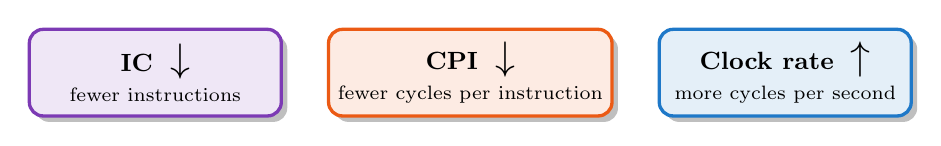
\begin{tikzpicture}
      \tikzset{kn/.style={very thick, rounded corners=5pt, minimum width=3.2cm, minimum height=1.1cm,
        align=center, font=\small, drop shadow}}
      \node[kn, draw=ProgramPurple, fill=ProgramPurple!12] at (0,0) {\textbf{IC} \ \Large$\downarrow$\\ \scriptsize fewer instructions};
      \node[kn, draw=AccentOrange, fill=AccentOrange!12] at (4,0) {\textbf{CPI} \ \Large$\downarrow$\\ \scriptsize fewer cycles per instruction};
      \node[kn, draw=StorageBlue, fill=StorageBlue!12] at (8,0) {\textbf{Clock rate} \ \Large$\uparrow$\\ \scriptsize more cycles per second};
    \end{tikzpicture}
  \end{center}
  \vspace{0.3cm}
  \begin{center}
    \large Improve \textbf{one} of the three\\[0.1cm]
    \large \textbf{without making the other two worse}.
  \end{center}
\end{frame}

\begin{frame}{What changes each of the three?}
  \begin{columns}[T,onlytextwidth]
    \column{0.31\textwidth}
      \begin{beamercolorbox}[rounded=true,sep=0.15cm,wd=\linewidth]{block body}
        \centering{\small\textbf{\textcolor{ProgramPurple}{IC}}}\\[0.05cm]
        {\Large\textcolor{ProgramPurple}{\faCode}}\par
        \footnotesize\raggedright
        \begin{itemize}\setlength{\itemsep}{2pt}
          \item the algorithm
          \item the compiler
          \item the instruction set (RISC or CISC)
        \end{itemize}
      \end{beamercolorbox}
    \column{0.31\textwidth}
      \begin{beamercolorbox}[rounded=true,sep=0.15cm,wd=\linewidth]{block body}
        \centering{\small\textbf{\textcolor{AccentOrange}{CPI}}}\\[0.05cm]
        {\Large\textcolor{AccentOrange}{\faProjectDiagram}}\par
        \footnotesize\raggedright
        \begin{itemize}\setlength{\itemsep}{2pt}
          \item the organisation of the processor: datapath, control unit
          \item e.g.\ \textbf{pipelining} (today!)
        \end{itemize}
      \end{beamercolorbox}
    \column{0.31\textwidth}
      \begin{beamercolorbox}[rounded=true,sep=0.15cm,wd=\linewidth]{block body}
        \centering{\small\textbf{\textcolor{StorageBlue}{Clock rate}}}\\[0.05cm]
        {\Large\textcolor{StorageBlue}{\faBolt}}\par
        \footnotesize\raggedright
        \begin{itemize}\setlength{\itemsep}{2pt}
          \item technology: faster transistors
          \item organisation: less work in each step
        \end{itemize}
      \end{beamercolorbox}
  \end{columns}
\end{frame}

% ---------- Exercise 1 ----------
\begin{frame}{Exercise 1: CPI of a MARIE program}
  \taskhead{Task}{A MARIE program executes $10^9$ instructions on a 1 GHz clock.}
  \begin{columns}[c,onlytextwidth]
    \column{0.52\textwidth}
      \centering
      \small
      \renewcommand{\arraystretch}{1.2}
      \begin{tabular}{lcc}
        \toprule
        Instruction & Share & Cycles \\
        \midrule
        \texttt{Load} & 30\% & 7 \\
        \texttt{Add} & 30\% & 7 \\
        \texttt{Store} & 20\% & 7 \\
        \texttt{Jump} & 10\% & 5 \\
        \texttt{Output} & 10\% & 5 \\
        \bottomrule
      \end{tabular}
    \column{0.44\textwidth}
      \begin{enumerate}\setlength{\itemsep}{8pt}
        \item What is the \textbf{average CPI}?
        \item What is the \textbf{execution time}?
      \end{enumerate}
      \vspace{0.3cm}
      \begin{beamercolorbox}[rounded=true,sep=0.1cm,wd=\linewidth]{block body}
        \scriptsize\textbf{Hint:} average CPI $= \sum_i \text{share}_i \times \text{cycles}_i$\\[2pt]
        1 GHz $= 10^9$ clock cycles per second
      \end{beamercolorbox}
  \end{columns}
\end{frame}

\begin{frame}{Solution: CPI of a MARIE program}
  \begin{center}
    \small
    \textbf{1. Average CPI}\\[0.15cm]
    $\text{CPI} = (0.3 + 0.3 + 0.2) \times 7 + (0.1 + 0.1) \times 5 = 5.6 + 1.0 = \mathbf{6.6}$\\[0.6cm]
    \textbf{2. Execution time}\\[0.15cm]
    $\text{CPU time} = \dfrac{\text{IC} \times \text{CPI}}{\text{clock rate}}
      = \dfrac{10^9 \times 6.6}{10^9\ \text{/s}} = \mathbf{6.6\ s}$
  \end{center}
\end{frame}

% ---------- Exercise 2 ----------
\begin{frame}{Exercise 2: the megahertz myth}
  \taskhead{Task}{Remember the two ARM processors from the beginning? The same program ($10^9$ instructions)
    and the same instruction set on two processors. The shop says: ``B has a 3 GHz clock instead of 2 GHz, so it is 1.5 times faster.''
    Is it true? Which one is faster, and how many times?}
  \vspace{0.2cm}
  \begin{columns}[T,onlytextwidth]
    \column{0.46\textwidth}
      \begin{beamercolorbox}[rounded=true,sep=0.16cm,wd=\linewidth]{block body}
        \centering\large\textbf{Processor A}\\[0.15cm]
        {\Huge\textcolor{DeepBlue}{\faMicrochip}}\\[0.15cm]
        \normalsize Clock: 2 GHz\\ CPI: 2.0
      \end{beamercolorbox}
    \column{0.46\textwidth}
      \begin{beamercolorbox}[rounded=true,sep=0.16cm,wd=\linewidth]{block body}
        \centering\large\textbf{Processor B}\\[0.15cm]
        {\Huge\textcolor{DeepBlue}{\faMicrochip}}\\[0.15cm]
        \normalsize Clock: 3 GHz\\ CPI: 3.5
      \end{beamercolorbox}
  \end{columns}
\end{frame}

\begin{frame}{Solution: the megahertz myth}
  \begin{columns}[c,onlytextwidth]
    \column{0.5\textwidth}
      \small
      \textbf{A:} $\dfrac{10^9 \times 2.0}{2 \times 10^9} = \mathbf{1.00\ s}$\\[0.3cm]
      \textbf{B:} $\dfrac{10^9 \times 3.5}{3 \times 10^9} = \mathbf{1.17\ s}$\\[0.3cm]
      $1.17 / 1.00 \approx 1.17$: \textbf{A is 1.17 times faster}.\\[0.3cm]
      The shop only divided the clock rates ($3 / 2 = 1.5$). It ignored CPI.
    \column{0.45\textwidth}
      \centering
      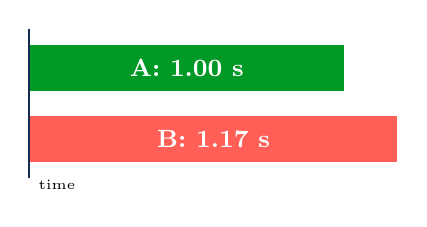
\begin{tikzpicture}
        \node[gbar, fill=mygreen, minimum width=4cm, minimum height=0.6cm, anchor=west, font=\small\bfseries] at (0,0) {A: 1.00 s};
        \node[gbar, fill=MacRed, minimum width=4.68cm, minimum height=0.6cm, anchor=west, font=\small\bfseries] at (0,-0.9) {B: 1.17 s};
        \draw[thick, DeepBlue] (0,0.5) -- (0,-1.4);
        \node[font=\tiny, anchor=north west] at (0,-1.3) {time};
      \end{tikzpicture}
  \end{columns}
  \vfill
  \keymsg{B has a faster clock but a worse CPI: improving one of the three is not enough if another one gets worse.}
\end{frame}

\begin{frame}{A popular number: MIPS}
  \begin{center}
    \Large
    $\text{MIPS} = \dfrac{\text{Instruction count}}{\text{Time} \times 10^6} = \dfrac{\text{Clock rate}}{\text{CPI} \times 10^6}$\\[0.2cm]
    \normalsize millions of instructions per second
  \end{center}
  \vspace{0.2cm}
  \begin{columns}[T,onlytextwidth]
    \column{0.48\textwidth}
      \stepbox{Why is it tempting?}{One number, and bigger means better.}
    \column{0.48\textwidth}
      \stepbox{A and B from Exercise 2}{A: 2000 / 2.0 = \textbf{1000 MIPS}\\ B: 3000 / 3.5 = \textbf{857 MIPS}\\
        MIPS agrees with time here.}
  \end{columns}
  \vfill
  \keymsg{Does MIPS \textbf{always} agree with execution time? Let's check.}
\end{frame}

% ---------- Exercise 3 ----------
\begin{frame}{Exercise 3: can MIPS lie?}
  \taskhead{Task}{Two processors, both 2 GHz, run the same program compiled for two
    \textbf{different instruction sets}. For each, compute the \textbf{execution time} and the \textbf{MIPS}.
    Which one is faster?}
  \vspace{0.3cm}
  \begin{center}
    \small
    \renewcommand{\arraystretch}{1.4}
    \begin{tabular}{lccc}
      \toprule
      Processor & Instruction count & CPI & Clock \\
      \midrule
      C (CISC) & $0.6 \times 10^9$ & 3.0 & 2 GHz \\
      D (RISC) & $2.0 \times 10^9$ & 1.0 & 2 GHz \\
      \bottomrule
    \end{tabular}
  \end{center}
\end{frame}

\begin{frame}{Solution: MIPS can lie}
  \begin{columns}[c,onlytextwidth]
    \column{0.52\textwidth}
      \centering
      \small
      \renewcommand{\arraystretch}{1.4}
      \begin{tabular}{lcc}
        \toprule
        & Time & MIPS \\
        \midrule
        C (CISC) & $\dfrac{0.6 \times 10^9 \times 3}{2 \times 10^9} = \textcolor{mygreen}{\mathbf{0.90\ s}}$ & 667 \\[0.3cm]
        D (RISC) & $\dfrac{2.0 \times 10^9 \times 1}{2 \times 10^9} = \mathbf{1.00\ s}$ & \textcolor{MacRed}{\textbf{2000}} \\
        \bottomrule
      \end{tabular}
    \column{0.44\textwidth}
      \stepbox{D has 3$\times$ more MIPS\ldots}{\ldots but C finishes the program first.}
      \stepbox{Why?}{MIPS ignores how much work one instruction does. Remember RISC vs CISC from Day 2.}
  \end{columns}
  \vfill
  \keymsg{Never compare MIPS across different instruction sets. \textbf{Compare time.}}
\end{frame}

\begin{frame}{How to compare fairly: benchmarks}
  \begin{columns}[c,onlytextwidth]
    \column{0.5\textwidth}
      \stepbox{Benchmark}{A real test program that we run on both processors. It measures \textbf{real work},
        not the number of instructions, so it cannot lie like MIPS.}
      \stepbox{Examples}{\textbf{SPEC CPU} for computers, \textbf{CoreMark} for microcontrollers.}
    \column{0.46\textwidth}
      \centering
      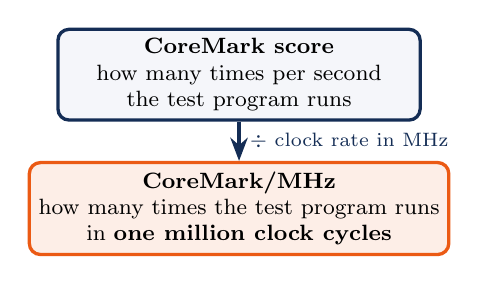
\begin{tikzpicture}
        \node[draw=DeepBlue, very thick, rounded corners=4pt, fill=LightGray, minimum width=4.6cm,
          minimum height=1.1cm, align=center, font=\footnotesize] (cm) at (0,0)
          {\textbf{CoreMark score}\\ how many times per second\\ the test program runs};
        \node[draw=AccentOrange, very thick, rounded corners=4pt, fill=AccentOrange!10, minimum width=4.6cm,
          minimum height=1.1cm, align=center, font=\footnotesize] (cmm) at (0,-1.7)
          {\textbf{CoreMark/MHz}\\ how many times the test program runs\\ in \textbf{one million clock cycles}};
        \draw[-{Stealth}, very thick, DeepBlue] (cm) -- node[right, font=\scriptsize] {$\div$ clock rate in MHz} (cmm);
      \end{tikzpicture}
  \end{columns}
  \vfill
  \keymsg{CoreMark/MHz lets us compare cores \textbf{independently of their clock rate}. Higher is better.}
\end{frame}

\begin{frame}{Back to the two ARM processors}
  \begin{center}
    \small
    \renewcommand{\arraystretch}{1.5}
    \begin{tabular}{lccc}
      \toprule
      & Clock rate & CoreMark/MHz & CoreMark score \\
      \midrule
      Arm Cortex-M3 (2004) & 120 MHz & 3.45 & $120 \times 3.45 \approx 414$ \\
      Arm Cortex-M7 (2014) & 100 MHz & 5.29 & $100 \times 5.29 \approx \mathbf{529}$ \\
      \bottomrule
    \end{tabular}\\[0.1cm]
    {\tiny\textcolor{gray}{Source: Arm Cortex-M Processor Comparison Table (2022), documentation-service.arm.com/static/61bb37962183326f2176f8cc}}
  \end{center}
  \vspace{0.2cm}
  \begin{center}
    \large $529 / 414 \approx \mathbf{1.28}$: the newer core is faster, with a \textbf{slower} clock.
  \end{center}
  \vfill
  \keymsg{Both cores use the same instruction set, so IC is about the same:
    the Cortex-M7 wins because it needs \textbf{fewer cycles per instruction}.}
\end{frame}

% ---------- Exercise 4 ----------
\begin{frame}{Exercise 4: write your own benchmark}
  \taskhead{Task}{Write a short Python program that does a \textbf{fixed amount} of work
    (for example arithmetic, strings or lists in a loop repeated N times) and measures \textbf{how long} it takes.}
  \footnotesize
  \begin{enumerate}\setlength{\itemsep}{3pt}
    \item Choose N so that the program runs \textbf{a few seconds} on your computer. Write N into the program.
    \item Run it 2--3 times. Write down the time, your \textbf{processor model}, its \textbf{clock rate}
      and your \textbf{Python version} (\mbox{\texttt{python -{}-version}}).
    \item Swap programs with your neighbour. Run \textbf{both} programs on \textbf{both} computers.
      \begin{itemize}\setlength{\itemsep}{1pt}
        \item How many times faster was one computer than the other in the first benchmark? And in the second?
        \item Did the same computer win in both benchmarks?
        \item Was the advantage similar in both, or clearly different?
      \end{itemize}
  \end{enumerate}
  \vfill
  \begin{beamercolorbox}[rounded=true,sep=0.1cm,wd=\textwidth]{block body}
    \scriptsize\textbf{Tips:} \texttt{time.perf\_counter()} gives the current time in seconds: read it before and after the work.
    Plug in your laptop and close other programs before you measure.
  \end{beamercolorbox}
\end{frame}

\begin{frame}[fragile]{Solution: an example benchmark}
  \begin{columns}[c,onlytextwidth]
    \column{0.55\textwidth}
\begin{lstlisting}[basicstyle=\color{VSText}\ttfamily\scriptsize]
import sys, time

N = 30_000_000        # fixed amount of work

start = time.perf_counter()
total = 0
for i in range(N):
    total += i * i % 7
end = time.perf_counter()

print("Python", sys.version.split()[0])
print(f"Time: {end - start:.2f} s")
\end{lstlisting}
    \column{0.41\textwidth}
      \stepbox{Fixed work, measured time}{The same N on every computer, so we compare the time of the same program.}
      \stepbox{Real benchmarks do the same}{SPEC CPU and CoreMark also run a fixed amount of work and measure the time.}
      \stepbox{Different benchmarks, different results}{The winner, or the size of the advantage, can change: a benchmark measures only the work it contains. That is why real suites like SPEC use many programs.}
  \end{columns}
\end{frame}


% =====================================================================
\section{From MARIE to RISC-V}
% =====================================================================

\begin{frame}{What is a datapath?}
  \begin{columns}[c,onlytextwidth]
    \column{0.6\textwidth}
      \centering
      \resizebox{\linewidth}{!}{\busdiagram{none}{none}{%
        \draw[AccentOrange, very thick, dashed, rounded corners=4pt] (-0.95,-0.9) rectangle (10.25,1.5);
        \node[font=\scriptsize\bfseries, text=AccentOrange, anchor=north] at (4.65,-0.95) {datapath};}}\\[0.1cm]
      \footnotesize\textbf{MARIE from Day 2:} the \textcolor{AccentOrange}{\textbf{datapath}} between
      the control unit and main memory
    \column{0.37\textwidth}
      \stepbox{Datapath}{The part of the processor where data \textbf{flows} and is \textbf{processed}:
        registers, ALU, connections to memory, buses and wires.}
      \stepbox{Control unit}{Tells the datapath \textbf{what to do} in every clock cycle:
        which register to read, what the ALU computes, whether to write.}
  \end{columns}
  \vfill
  \keymsg{Processor = \textbf{datapath} + \textbf{control unit}.}
\end{frame}

\begin{frame}{Why leave MARIE?}
  \begin{columns}[c,onlytextwidth]
    \column{0.62\textwidth}
      \centering
      \resizebox{\linewidth}{!}{\busdiagram{none}{none}{%
        \draw[MacRed, very thick, rounded corners=3pt] (0.3,-0.6) rectangle (10.6,-0.1);
        \node[font=\scriptsize\bfseries, text=MacRed, anchor=north] at (5.5,-0.65) {one bus for everything};}}
    \column{0.35\textwidth}
      \stepbox{One bus}{Only one value can travel at a time.}
      \stepbox{One accumulator}{Almost every instruction needs AC, so instructions always wait for each other.}
      \stepbox{What we need}{Separate paths for instructions and data, and many registers.}
  \end{columns}
  \vfill
  \keymsg{We switch to \textbf{RISC-V}: the RISC idea from Day 2 made real.}
\end{frame}

\begin{frame}{Meet RISC-V}
  \begin{columns}[c,onlytextwidth]
    \column{0.35\textwidth}
      \centering
      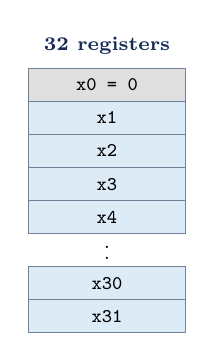
\begin{tikzpicture}
        \foreach \t [count=\i from 0] in {x0,x1,x2,x3,x4,\vdots,x30,x31} {
          \ifnum\i=5
            \node[font=\scriptsize] at (0,{-0.42*\i}) {$\vdots$};
          \else
            \ifnum\i=0
              \node[mcell, minimum width=2cm, fill=gray!25] at (0,{-0.42*\i}) {\t\ = 0};
            \else
              \node[mcell, minimum width=2cm] at (0,{-0.42*\i}) {\t};
            \fi
          \fi
        }
        \node[font=\scriptsize\bfseries, text=DeepBlue] at (0,0.5) {32 registers};
      \end{tikzpicture}
    \column{0.6\textwidth}
      \stepbox{32 registers}{\texttt{x0} \dots\ \texttt{x31}, 32 bits each. \texttt{x0} is always 0.}
      \stepbox{Load/store architecture}{Memory is used only by \texttt{lw} (load word) and \texttt{sw} (store word).
        Arithmetic works on registers.}
      \stepbox{Fixed length}{Every instruction is exactly 32 bits long.}
  \end{columns}
  \vfill
  \keymsg{An \textbf{open} instruction set: used in teaching, in microcontrollers, and more and more in industry.}
\end{frame}

\begin{frame}[fragile]{The same program twice: $Z = X + Y$}
  \begin{columns}[T,onlytextwidth]
    \column{0.36\textwidth}
      \centering\footnotesize\textbf{MARIE}\\[0.05cm]
\begin{lstlisting}[style=marie, numbers=none]
Load X
Add Y
Store Z
Halt
X, Dec 1
Y, Dec 2
Z, Dec 0
\end{lstlisting}
    \column{0.52\textwidth}
      \centering\footnotesize\textbf{RISC-V}\\[0.05cm]
\begin{lstlisting}[style=rv]
.data
X: .word 1
Y: .word 2
Z: .word 0
.text
lw  x5, X          # x5 = X
lw  x6, Y          # x6 = Y
add x7, x5, x6     # x7 = X + Y
sw  x7, Z, x28     # Z = x7
\end{lstlisting}
  \end{columns}
\end{frame}

\begin{frame}{Three more instructions}
  \begin{center}
    \small
    \renewcommand{\arraystretch}{1.5}
    \begin{tabular}{ll}
      \toprule
      Instruction & Meaning \\
      \midrule
      \texttt{addi x7, x7, -2} & \mo{x7}{x7 $-$ 2} \quad (a constant inside the instruction) \\
      \texttt{beq\ \ x5, x6, label} & if \texttt{x5} = \texttt{x6}, jump to \texttt{label} \\
      \texttt{bnez x5, label} & if \texttt{x5} $\neq$ 0, jump to \texttt{label} \\
      \bottomrule
    \end{tabular}\\[0.3cm]
    \footnotesize\textcolor{gray}{Already known: \texttt{lw}, \texttt{sw}, \texttt{add}}
  \end{center}
  \vfill
  \keymsg{\texttt{beq} and \texttt{bnez} are \textbf{branches}: MARIE's \texttt{Skipcond} and \texttt{Jump} in one instruction.}
\end{frame}

% ---------- Exercise 5 ----------
\begin{frame}{Now a simulator is the CPU: Ripes}
  \begin{center}
    \small We will run our RISC-V programs in a simulator, in the browser:\\[0.6cm]
    {\Huge\textcolor{DeepBlue}{\faGlobe}}\\[0.3cm]
    \LARGE\texttt{https://ripes.dk}
    % A real screenshot can be added here:
    % \\[0.3cm]\includegraphics[width=0.6\textwidth]{ripes.png}
  \end{center}
\end{frame}

\begin{frame}{Exercise 5: your first RISC-V program}
  \begin{columns}[T,onlytextwidth]
    \column{0.58\textwidth}
      \taskhead{Ripes task}{Write $Z = (X + Y) - 2$ in RISC-V and run it in Ripes.}
      \footnotesize
      \begin{itemize}\setlength{\itemsep}{3pt}
        \item Put \texttt{X: .word 5}, \texttt{Y: .word 3} and \texttt{Z: .word 0} in the \texttt{.data} part.
        \item Use only the instructions we have seen: \texttt{lw}, \texttt{sw}, \texttt{add}, \texttt{addi}.
        \item Before running, choose the \textbf{single-cycle processor} (\textcolor{DeepBlue}{\faMicrochip}).
      \end{itemize}
    \column{0.38\textwidth}
      \stepbox{Day 2}{You solved this in ``RISC style'' with \texttt{load}, \texttt{add}, \texttt{sub} and \texttt{store}.
        Now it is a real instruction set.}
  \end{columns}
\end{frame}

\begin{frame}[fragile]{Solution: your first RISC-V program}
  \begin{center}
    \begin{minipage}{0.55\textwidth}
\begin{lstlisting}[style=rv]
.data
X: .word 5
Y: .word 3
Z: .word 0
.text
lw   x5, X          # x5 = X
lw   x6, Y          # x6 = Y
add  x7, x5, x6     # x7 = X + Y
addi x7, x7, -2     # x7 = x7 - 2
sw   x7, Z, x28     # Z = x7
\end{lstlisting}
    \end{minipage}
  \end{center}
\end{frame}

% ---------- Exercise 6 ----------
\begin{frame}[fragile]{Exercise 6: your first branch}
  \begin{columns}[T,onlytextwidth]
    \column{0.55\textwidth}
      \taskhead{Ripes task}{Write a program that sets \texttt{Z} = 1 if \texttt{X} = \texttt{Y},
        and \texttt{Z} = 0 otherwise.}
      \footnotesize
      \begin{itemize}\setlength{\itemsep}{4pt}
        \item Use \texttt{beq} from the table: if two registers are equal, jump to a label.
        \item Run it twice: with \texttt{X} = 5, \texttt{Y} = 5 and with \texttt{X} = 5, \texttt{Y} = 3.
          Check \texttt{Z} in the \textbf{Memory} tab.
      \end{itemize}
    \column{0.41\textwidth}
      \stepbox{Day 2}{In MARIE you did this with \texttt{Skipcond}: skip the next instruction if a condition is true.}
      \begin{beamercolorbox}[rounded=true,sep=0.1cm,wd=\linewidth]{block body}
        \scriptsize\textbf{Hint:} a label marks a line: \texttt{done: sw x7, Z, x28}.
        \texttt{beq x5, x6, done} jumps there.
      \end{beamercolorbox}
  \end{columns}
\end{frame}

\begin{frame}[fragile]{Solution: your first branch}
  \begin{columns}[c,onlytextwidth]
    \column{0.56\textwidth}
\begin{lstlisting}[style=rv]
.data
X: .word 5
Y: .word 5
Z: .word 0
.text
      lw   x5, X
      lw   x6, Y
      addi x7, x0, 1       # guess: equal, Z = 1
      beq  x5, x6, done    # if X = Y, skip next line
      addi x7, x0, 0       # not equal, Z = 0
done: sw   x7, Z, x28
\end{lstlisting}
    \column{0.4\textwidth}
      \stepbox{X = 5, Y = 5}{\texttt{beq} jumps to \texttt{done}: \texttt{Z} = \textbf{1}}
      \stepbox{X = 5, Y = 3}{no jump, the next line runs: \texttt{Z} = \textbf{0}}
  \end{columns}
  \vfill
  \keymsg{\texttt{beq} decides which instruction comes next. Remember this: it will matter in the last part of today.}
\end{frame}

\begin{frame}{Five steps of every instruction}
  \begin{center}
    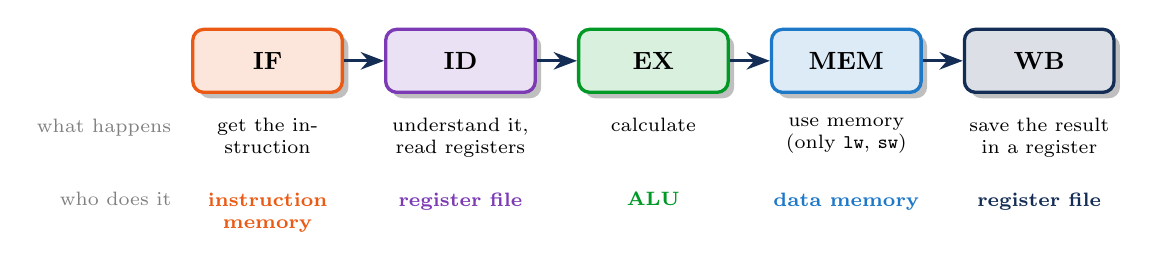
\begin{tikzpicture}[>=Stealth]
      \foreach \n/\c/\w/\h [count=\i from 0] in {
          IF/cIF/get the instruction/instruction memory,
          ID/cID/understand it{,} read registers/register file,
          EX/cEX/calculate/ALU,
          MEM/cMEM/use memory (only \texttt{lw}{,} \texttt{sw})/data memory,
          WB/cWB/save the result in a register/register file} {
        \node[stagebox, draw=\c, fill=\c!15] (s\i) at ({2.45*\i},0) {\n};
        \node[font=\scriptsize, align=center, text width=2.2cm, anchor=north] (t\i) at ({2.45*\i},-0.6) {\w};
        \node[font=\scriptsize\bfseries, align=center, text width=2.2cm, anchor=north, text=\c] at ({2.45*\i},-1.55) {\h};
      }
      \foreach \i [evaluate=\i as \j using int(\i+1)] in {0,...,3}
        \draw[->, very thick, DeepBlue] (s\i) -- (s\j);
      \node[font=\scriptsize, text=gray, anchor=east] at (-1.1,-0.85) {what happens};
      \node[font=\scriptsize, text=gray, anchor=east] at (-1.1,-1.75) {who does it};
    \end{tikzpicture}
  \end{center}
  \vfill
  \keymsg{Each step uses a \textbf{different part} of the processor.}
\end{frame}

\begin{frame}{Single-cycle: one instruction per clock cycle}
  \begin{center}
    \small
    \renewcommand{\arraystretch}{1.3}
    \begin{tabular}{ccccc}
      \toprule
      \textcolor{cIF}{\textbf{IF}} & \textcolor{cID}{\textbf{ID}} & \textcolor{cEX}{\textbf{EX}} & \textcolor{cMEM}{\textbf{MEM}} & \textcolor{cWB}{\textbf{WB}} \\
      \midrule
      200 ps & 100 ps & 200 ps & 200 ps & 100 ps \\
      \bottomrule
    \end{tabular}\\[0.05cm]
    {\tiny typical textbook values; 1 ps = $10^{-12}$ s}
  \end{center}
  \vspace{0.2cm}
  \begin{center}
    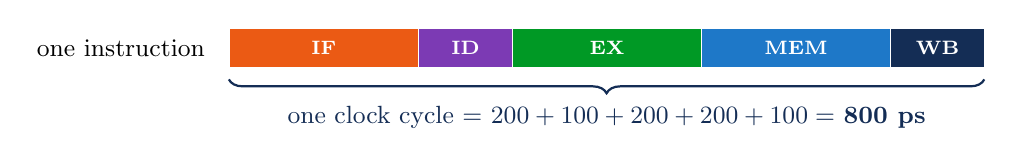
\begin{tikzpicture}[x=0.012cm]
      \def\acc{0}
      \foreach \s/\t in {IF/200,ID/100,EX/200,MEM/200,WB/100} {
        \node[gbar, fill=c\s, minimum width=\t*0.012 cm, anchor=west, minimum height=0.5cm, font=\scriptsize\bfseries] at (\acc,0) {\s};
        \pgfmathparse{\acc+\t}\xdef\acc{\pgfmathresult}
      }
      \draw[decorate, decoration={brace, amplitude=5pt, mirror}, thick, DeepBlue] (0,-0.4) -- (800,-0.4)
        node[midway, below=6pt, font=\small] {one clock cycle = $200 + 100 + 200 + 200 + 100 =$ \textbf{800 ps}};
      \node[anchor=east, font=\small] at (-15,0) {one instruction};
    \end{tikzpicture}
  \end{center}
  \vfill
  \keymsg{The whole instruction must fit into \textbf{one} clock cycle, so the cycle is long: \textbf{800 ps}.}
\end{frame}

% =====================================================================
\section{Pipelining}
% =====================================================================

\begin{frame}{One instruction at a time}
  \begin{center}
    \small Three instructions on the \textbf{single-cycle} processor: $3 \times 800$ ps = 2400 ps.\\[0.25cm]
    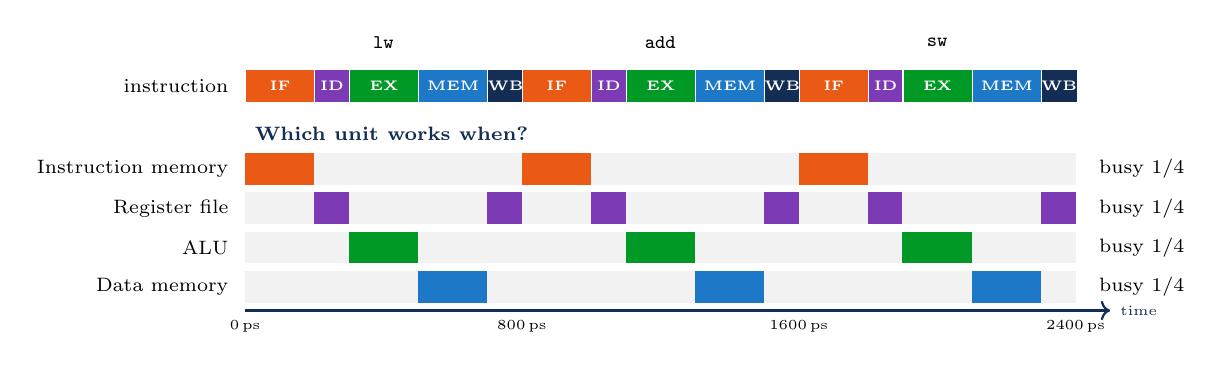
\begin{tikzpicture}[x=0.0044cm]
      % instructions
      \foreach \ins [count=\k from 0] in {lw, add, sw} {
        \pgfmathsetmacro{\off}{800*\k}
        \node[font=\ttfamily\scriptsize] at (\off+400,0.55) {\ins};
        \def\acc{\off}
        \foreach \s/\t in {IF/200,ID/100,EX/200,MEM/200,WB/100} {
          \node[gbar, fill=c\s, minimum width=\t*0.0044 cm, anchor=west, minimum height=0.42cm, font=\tiny\bfseries] at (\acc,0) {\s};
          \pgfmathparse{\acc+\t}\xdef\acc{\pgfmathresult}
        }
      }
      \node[anchor=east, font=\scriptsize] at (-20,0) {instruction};
      % unit usage
      \node[font=\scriptsize\bfseries, text=DeepBlue, anchor=west] at (0,-0.6) {Which unit works when?};
      \foreach \u/\c/\list [count=\r from 1] in {
          Instruction memory/cIF/{0},
          Register file/cID/{200,700},
          ALU/cEX/{300},
          Data memory/cMEM/{500}} {
        \pgfmathsetmacro{\y}{-0.55-0.5*\r}
        \node[anchor=east, font=\scriptsize] at (-20,\y) {\u};
        \fill[gray!10] (0,\y-0.2) rectangle (2400,\y+0.2);
        \foreach \k in {0,1,2}
          \foreach \st in \list {
            \pgfmathsetmacro{\w}{(\st==200 || \st==700) ? 100 : 200}
            \fill[\c] ({800*\k+\st},\y-0.2) rectangle ({800*\k+\st+\w},\y+0.2);
          }
        \node[anchor=west, font=\scriptsize] at (2440,\y) {busy 1/4};
      }
      \draw[->, thick, DeepBlue] (0,-2.85) -- (2500,-2.85) node[right, font=\tiny] {time};
      \foreach \t in {0,800,1600,2400} \node[font=\tiny, below] at (\t,-2.85) {\t\,ps};
    \end{tikzpicture}
  \end{center}
  \vspace{-0.1cm}
  \begin{center}
    \large\textbf{Every unit is idle most of the time. Could these steps overlap?}
  \end{center}
\end{frame}

\begin{frame}{The laundry problem}
  \begin{center}
    \small 4 loads of laundry. Each load needs 4 steps of 30 minutes:
    \textcolor{cIF}{\textbf{wash}}, \textcolor{cID}{\textbf{dry}}, \textcolor{cEX}{\textbf{fold}}, \textcolor{cMEM}{\textbf{put away}}.\\[0.35cm]
    \begin{tikzpicture}[x=0.72cm]
      \foreach \l in {0,...,3} {
        \node[anchor=east, font=\scriptsize] at (-0.2,{-0.55*\l}) {\textcolor{DeepBlue}{\faTshirt}\ load \the\numexpr\l+1\relax};
        \foreach \s/\c [count=\k from 0] in {W/cIF, D/cID, F/cEX, P/cMEM}
          \node[gbar, fill=\c, minimum width=0.72cm, minimum height=0.42cm, font=\tiny\bfseries] at ({4*\l+\k+0.5},{-0.55*\l}) {\s};
      }
      \draw[->, thick, DeepBlue] (0,-2.1) -- (16.3,-2.1);
      \foreach \h in {0,...,8} {
        \draw[thick, DeepBlue] ({2*\h},-2.05) -- ({2*\h},-2.15);
        \node[font=\tiny, below] at ({2*\h},-2.1) {\h\,h};
      }
    \end{tikzpicture}
  \end{center}
  \vfill
  \keymsg{One load at a time: \textbf{8 hours}. The washing machine works only 1/4 of the time.}
\end{frame}

\begin{frame}{Decision: start the next load early}
  \begin{center}
    \small As soon as the washing machine is free, put the next load in.\\[0.35cm]
    \begin{tikzpicture}[x=0.72cm]
      \fill[AccentOrange!12] (3,0.35) rectangle (4,-2.0);
      \foreach \l in {0,...,3} {
        \node[anchor=east, font=\scriptsize] at (-0.2,{-0.55*\l}) {\textcolor{DeepBlue}{\faTshirt}\ load \the\numexpr\l+1\relax};
        \foreach \s/\c [count=\k from 0] in {W/cIF, D/cID, F/cEX, P/cMEM}
          \node[gbar, fill=\c, minimum width=0.72cm, minimum height=0.42cm, font=\tiny\bfseries] at ({\l+\k+0.5},{-0.55*\l}) {\s};
      }
      \node[font=\tiny\bfseries, text=AccentOrange, anchor=west] at (7.3,-0.8) {$\leftarrow$ all four machines busy};
      \node[font=\tiny\bfseries, text=AccentOrange, anchor=south] at (3.5,0.35) {};
      \draw[->, thick, DeepBlue] (0,-2.1) -- (16.3,-2.1);
      \foreach \h in {0,...,8} {
        \draw[thick, DeepBlue] ({2*\h},-2.05) -- ({2*\h},-2.15);
        \node[font=\tiny, below] at ({2*\h},-2.1) {\h\,h};
      }
      \draw[<->, thick, mygreen] (0,-2.75) -- node[below, font=\scriptsize\bfseries] {3.5 h} (7,-2.75);
    \end{tikzpicture}
  \end{center}
  \vfill
  \keymsg{\textbf{3.5 hours.} Each load still takes 2 hours, but one load is finished \textbf{every 30 minutes}.}
\end{frame}

\begin{frame}{Pipelining instructions}
  \begin{center}
    \small A new instruction starts every cycle. Each cycle, every instruction moves one stage forward.\\[0.3cm]
    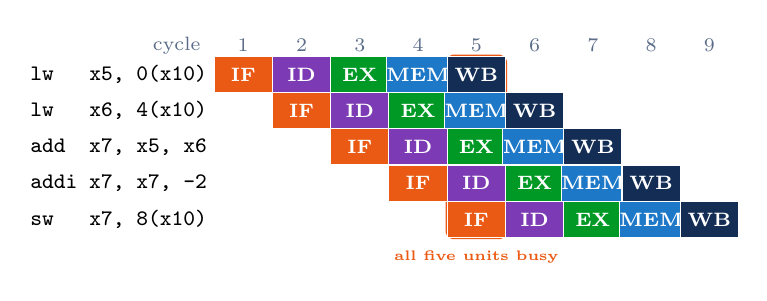
\begin{tikzpicture}
      \pcycles{9}
      \pcolumn{5}{5}{AccentOrange}
      \plabel{0}{lw\ \ \ x5, 0(x10)} \prow{0}{1}{IF,ID,EX,MEM,WB}
      \plabel{1}{lw\ \ \ x6, 4(x10)} \prow{1}{2}{IF,ID,EX,MEM,WB}
      \plabel{2}{add\ \ x7, x5, x6}  \prow{2}{3}{IF,ID,EX,MEM,WB}
      \plabel{3}{addi x7, x7, -2}    \prow{3}{4}{IF,ID,EX,MEM,WB}
      \plabel{4}{sw\ \ \ x7, 8(x10)} \prow{4}{5}{IF,ID,EX,MEM,WB}
      \node[font=\tiny\bfseries, text=AccentOrange, anchor=north] at ({4*\pw},{-4.6*\ph}) {all five units busy};
    \end{tikzpicture}\\[0.2cm]
    \stagelegend
  \end{center}
  \vfill
  \keymsg{After the pipeline fills up, \textbf{one instruction finishes every cycle}.}
  \simfoot{\simlink{pipeline}}
\end{frame}

% ---------- Exercise 7 ----------
\begin{frame}[fragile]{Exercise 7: watch the pipeline}
  \begin{columns}[T,onlytextwidth]
    \column{0.36\textwidth}
\begin{lstlisting}[style=rv]
addi x5, x0, 1
addi x6, x0, 2
addi x7, x0, 3
addi x8, x0, 4
addi x9, x0, 5
\end{lstlisting}
      \vspace{0.1cm}
      \scriptsize\textcolor{gray}{\texttt{x0} is always 0, so \texttt{addi x5, x0, 1} puts 1 into \texttt{x5}.}
    \column{0.6\textwidth}
      \taskhead{Ripes task}{Choose the \textbf{5-stage processor} (\textcolor{DeepBlue}{\faMicrochip}).
        Run the program one step at a time and watch the \textbf{Editor}: the coloured bars show
        which instruction is in which stage.}
      \footnotesize
      \begin{enumerate}\setlength{\itemsep}{4pt}
        \item What is the largest number of instructions in the processor at the same time?
        \item After how many steps does the first instruction finish (WB)? And the last one?
        \item How many cycles and instructions does Ripes count?
      \end{enumerate}
  \end{columns}
  \simfoot{\simlink{pipeline}}
\end{frame}

\begin{frame}{Solution: watch the pipeline}
  \begin{center}
    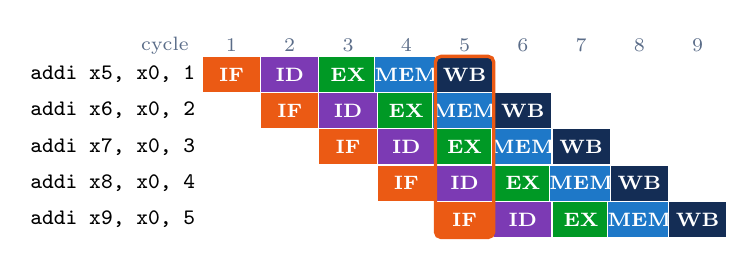
\begin{tikzpicture}
      \pcycles{9}
      \plabel{0}{addi x5, x0, 1} \prow{0}{1}{IF,ID,EX,MEM,WB}
      \plabel{1}{addi x6, x0, 2} \prow{1}{2}{IF,ID,EX,MEM,WB}
      \plabel{2}{addi x7, x0, 3} \prow{2}{3}{IF,ID,EX,MEM,WB}
      \plabel{3}{addi x8, x0, 4} \prow{3}{4}{IF,ID,EX,MEM,WB}
      \plabel{4}{addi x9, x0, 5} \prow{4}{5}{IF,ID,EX,MEM,WB}
      \pcolumn{5}{5}{AccentOrange}
    \end{tikzpicture}
  \end{center}
  \vspace{-0.1cm}
  \begin{columns}[T,onlytextwidth]
    \column{0.31\textwidth}
      \stepbox{1. At the same time}{up to \textbf{5} instructions (step 5)}
    \column{0.31\textwidth}
      \stepbox{2. Finished}{the first after \textbf{5} steps, the last after \textbf{9}}
    \column{0.31\textwidth}
      \stepbox{3. Ripes}{\textbf{9 cycles}, \textbf{5 instructions}}
  \end{columns}
  \vfill
  \keymsg{After the pipeline fills up, \textbf{one instruction finishes every cycle}.}
\end{frame}

% =====================================================================
\section{Branches}
% =====================================================================

\begin{frame}[fragile]{Control hazard: which instruction comes next?}
  \begin{columns}[c,onlytextwidth]
    \column{0.42\textwidth}
\begin{lstlisting}[style=rv]
      li   x11, 3
loop: addi x11, x11, -1
      bnez x11, loop
      addi x12, x0, 7
\end{lstlisting}
      \vspace{0.1cm}
      \stepbox{The problem}{The pipeline fetches a new instruction \textbf{every cycle}.
        But after \texttt{bnez}: the next line, or back to \texttt{loop}?}
    \column{0.54\textwidth}
      \centering
      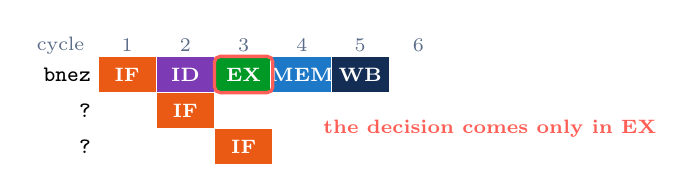
\begin{tikzpicture}
        \pcycles{6}
        \plabel{0}{bnez}  \prow{0}{1}{IF,ID,EX,MEM,WB}
        \plabel{1}{?}     \prow{1}{2}{IF}
        \plabel{2}{?}     \prow{2}{3}{IF}
        \draw[MacRed, very thick, rounded corners=2pt] ({1.5*\pw},{0.5*\ph}) rectangle ({2.5*\pw},{-0.5*\ph});
        \node[font=\scriptsize\bfseries, text=MacRed, anchor=west] at ({3.2*\pw},{-1.5*\ph}) {the decision comes only in EX};
      \end{tikzpicture}
  \end{columns}
  \vfill
  \keymsg{When \texttt{bnez} finally knows the answer, \textbf{two more instructions} are already in the pipeline.}
\end{frame}

\begin{frame}{Fetch anyway, throw away if wrong}
  \begin{columns}[c,onlytextwidth]
    \column{0.55\textwidth}
      \centering
      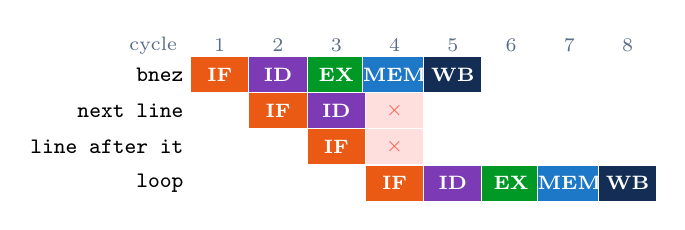
\begin{tikzpicture}
        \pcycles{8}
        \plabel{0}{bnez}          \prow{0}{1}{IF,ID,EX,MEM,WB}
        \plabel{1}{next line}     \prow{1}{2}{IF,ID,X}
        \plabel{2}{line after it} \prow{2}{3}{IF,X}
        \plabel{3}{loop}          \prow{3}{4}{IF,ID,EX,MEM,WB}
      \end{tikzpicture}
    \column{0.42\textwidth}
      \stepbox{Simplest idea}{Keep fetching the next lines, as if there were no jump.}
      \stepbox{If the jump happens}{Throw the fetched instructions away (\textbf{flush}) and start again at \texttt{loop}.}
  \end{columns}
  \vfill
  \keymsg{Each jump costs \textbf{2 cycles}: two instructions were started for nothing.}
\end{frame}

% ---------- Exercise 8 ----------
\begin{frame}[fragile]{Exercise 8: catch the flush}
  \begin{columns}[T,onlytextwidth]
    \column{0.42\textwidth}
\begin{lstlisting}[style=rv]
      li   x11, 3          # counter = 3
loop: addi x11, x11, -1    # counter - 1
      bnez x11, loop       # repeat while != 0
      addi x12, x0, 7      # after the loop
\end{lstlisting}
    \column{0.54\textwidth}
      \taskhead{Ripes task}{5-stage processor. Run the program one step at a time and watch
        the last line, \texttt{addi x12, x0, 7}, in the \textbf{Editor}.}
      \footnotesize
      \begin{enumerate}\setlength{\itemsep}{4pt}
        \item How many times does \texttt{addi x12} enter the pipeline (IF) before it finally reaches WB?
        \item What happens to it the other times? Why?
        \item How many times does the loop jump back?
      \end{enumerate}
  \end{columns}
  \simfoot{\simlink{pipeline}}
\end{frame}

\begin{frame}{Solution: catch the flush}
  \begin{center}
    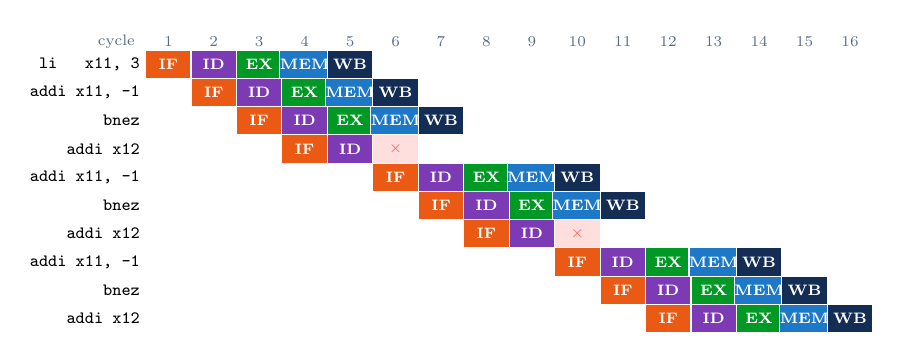
\begin{tikzpicture}[scale=0.78, every node/.style={transform shape}]
      \pcycles{16}
      \plabel{0}{li\ \ \ x11, 3}     \prow{0}{1}{IF,ID,EX,MEM,WB}
      \plabel{1}{addi x11, -1}       \prow{1}{2}{IF,ID,EX,MEM,WB}
      \plabel{2}{bnez}               \prow{2}{3}{IF,ID,EX,MEM,WB}
      \plabel{3}{addi x12}           \prow{3}{4}{IF,ID,X}
      \plabel{4}{addi x11, -1}       \prow{4}{6}{IF,ID,EX,MEM,WB}
      \plabel{5}{bnez}               \prow{5}{7}{IF,ID,EX,MEM,WB}
      \plabel{6}{addi x12}           \prow{6}{8}{IF,ID,X}
      \plabel{7}{addi x11, -1}       \prow{7}{10}{IF,ID,EX,MEM,WB}
      \plabel{8}{bnez}               \prow{8}{11}{IF,ID,EX,MEM,WB}
      \plabel{9}{addi x12}           \prow{9}{12}{IF,ID,EX,MEM,WB}
    \end{tikzpicture}
  \end{center}
  \vspace{-0.15cm}
  \begin{columns}[T,onlytextwidth]
    \column{0.48\textwidth}
      \stepbox{1--2. Three times}{Twice it is \textbf{thrown away}: \texttt{bnez} decided to jump back to \texttt{loop}.}
    \column{0.48\textwidth}
      \stepbox{3. Two jumps}{The third time \texttt{x11} = 0, so there is no jump and \texttt{addi x12} finishes.}
  \end{columns}
\end{frame}

\begin{frame}{Processors guess}
  \begin{columns}[c,onlytextwidth]
    \column{0.5\textwidth}
      \stepbox{Always ``next line''}{is a bad guess for a loop: a loop almost always jumps back.}
      \stepbox{Branch prediction}{The processor remembers what each branch did \textbf{last time} and fetches from there.}
      \stepbox{In real processors}{The guess is right \textbf{well over 90\%} of the time.}
    \column{0.46\textwidth}
      \centering
      \begin{tikzpicture}[>=Stealth]
        \node[draw=DeepBlue, very thick, rounded corners=4pt, fill=LightGray, align=center, font=\footnotesize,
          minimum width=3.6cm, minimum height=1cm] (b) at (0,0) {\texttt{bnez x11, loop}};
        \node[draw=mygreen, very thick, rounded corners=4pt, fill=mygreen!10, align=center, font=\footnotesize,
          minimum width=3.6cm, minimum height=1cm] (m) at (0,-1.8) {last time: \textbf{jumped}\\ guess: jump again};
        \draw[->, very thick, DeepBlue] (b) -- node[right, font=\scriptsize] {remember} (m);
        \node[font=\Huge, text=mygreen] at (2.4,-1.8) {\faCheck};
      \end{tikzpicture}
  \end{columns}
  \vfill
  \keymsg{A good guess means the loop loses cycles only once: when it finally \textbf{leaves} the loop.}
\end{frame}
\end{document}